\documentclass[12pt,openany]{book}
%\usepackage{classnotestikz}
%\usepackage{tikzelements}
\usepackage{libro-fciencias}
\usepackage{booktabs}
\usepackage{colortbl}
\def\thickline{\specialrule{.15em}{.05em}{.05em}}
\def\violetrule{\color{Violeta}{\rule{100px}{0.05em}}}
\def\bluerule{\color{DarkBlue}{\rule{100px}{0.05em}}}
\usepackage{multirow}


\usepackage{diagramas-fciencias}
\pgfplotsset{compat=1.15}

\graphicspath{ {Figuras/} }

%\setcounter{tocdepth}{4}

\addbibresource{rnnotesref.bib}


%----------------------------------------------------------------------------------------
%	Autores y Título
%----------------------------------------------------------------------------------------

\title{Redes Neuronales}
\subtitle{Notas de clase}
\author{Karla Fernanda Jiménez Gutiérrez\newline
        Verónica Esther Arriola Ríos}
\publisher{Facultad de Ciencias, UNAM}
\background{Neurona.png}


\begin{document}
\maketitle

%----------------------------------------------------------------------------------------
% Contenido
%----------------------------------------------------------------------------------------
\frontmatter % Numeración romana
\tableofcontents
\clearemptydoublepage % Whitespace to the end of the page


%----------------------------------------------------------------------------------------
%	                                Inicio
%----------------------------------------------------------------------------------------
\mainmatter  % Numeración arabiga


%%
\chapter*{Etc}

A lo largo del texto se utilizará la siguiente notación para diversos elementos:
\begin{longtable}{lc}
 Conjuntos   &   $\set{C}$ \\
 Vectores    &   $\vec{X}$ \\
 Matrices    &   $\mat{M}$ \\
 Unidades    &   $\unit{cm}$
\end{longtable}



%%
\part{Antecedentes}
\chapter{Neurona biológica}
\section{Neurociencias computacionales}

El campo conocido como \textbf{neurociencias computacionales}\cite{sonNC} es el que se dedica explícitamente al estudio/modelado de los sistemas biológicos con ayuda de varios campos de estudio. Se interesa notablemente en descripciones y modelos funcionales biológicamente realistas de neuronas y sistemas neuronales. 

Los campos de estudio de los cuales nos ayudamos son:
\begin{itemize}
 \item  \textbf{Ciencias cognitivas} dedicadas a tratar directamente con los humanos, de estás tomamos los conceptos de aprendizaje.
 \item  \textbf{Biofísica}  por el estudio de las propiedades físicas en de los sistemas biológicos. 
 \item  \textbf{Neurociencias tradicionales} con modelos matemáticos. 
 
 \item  \textbf{Ciencias de la computación} modelar e implementar los modelos dados, por las aréas aquí listadas. Simulaciones computacionales. 
 
 \item  \textbf{Ingeniería eléctrica} diseño de hardware especifico y eficiente para tomar los pulsos y medidas exactas.  
 
\end{itemize}

Las neurociencias computacionales, estudian modelos del sistema nervioso y clasifican estos modelos en tres tipos, recordemos el método cientifico: 

\begin{enumerate}
 \item \textbf{Modelos descriptivos}, Describen. Por ejemplo describe el comportamiento de los ratones a ciertas sustancias. La \textbf{comparación}, que estaba pasando antes de la sustancia, con la sustancia y después. 
  
 \item \textbf{Modelos mecanistas}, Mecánicamente. El \textbf{cómo} paso el evento o la acción. Siguiendo con el ejemplo. El ratón se cayo y se levanto, ¿Cómo? Doblo sus articulaciones, tomo impulso con sus musculos, roto su cuerpo, hasta reicorporarse totalmente.
 
 \item \textbf{Modelos interpretativos}, Se interpreta. ¿\textbf{Porque} hizo los movimientos mecanicos?. Siguiendo con el ejemplo. ¿Porque el ratón se reincorporo? Porque el ratón quiere regresar a su estado anterior antes de la pertubación por la sustancia. ¿Sera verdad? Es lo que se interpreta, no la verdad absoluta. Se tiene que buscar intencionalidad, razonamiento de más alto nivel.
 
\end{enumerate}

Los \textbf{objetivos del modelado} en neurociencias de nuestro interes en el curso son; Las corrientes, las proteínas, las oscilaciones de las redes completa, la arquitectura topografica y de columnas, el aprendizaje y la memoria. Por lo menos para el curso de Redes Neuronales en la Universidad Nacional Autonoma de México con la profesora Veronica Arriola Rios.

Para más información en Neurociencias \cite{princNS5}, siempre está el interes propio.

Las redes neuronales artificiales (RNA), estan inspiradas en las redes neuronales biológicas, tales como las de los animales \cite{incipiencias}, en un primer momento. Hasta llegar al ser humano con el sistema nervioso y nuestras neuronas. \cite{ideaNeurona}. 

Los modelos de redes neuronales que tomaremos, son simples. Distan mucho de los sistemas naturales y aun así dan solución. Lo que nos interesa es que resuelvan los problemas inmediatos y de corto plazo. Si el cerebro humano funciona, la imitación debe darnos algunos resultados, idea que ha funcionado para procesar información y dar solución con modelos diseñados. 

Los problemas más notorios a resolver son: 
\begin{itemize}
\item Problemas de visión por computadora.
\item Procesamiento del lenguaje natural.
\end{itemize}

\section{Sistema Nervioso}


\textbf{¿Qué son las neuronas?} 
Las neuronas son células con núcleo, sus cuerpos tienen dendritas con la habilidad de transferir electricidad y un axón.  Éste es una terminal eferente, que permite transmitir un pulso eléctrico desde el cuerpo a través del axón hasta otras neuronas a distancias variadas.


\textbf{¿Qué es un nervio?}
Un nervio es una gran colección de axones empacados todos juntos en una especie de cable (fibra), pasan vasos sanguíneos por en medio de los nervios. Esto es de lo que está formando el sistema nervioso, se originan desde la médula espinal (31 pares de nervios raquídeos) o el encéfalo (12 pares de nervios craneales).


Los nervios son estructuras conductoras de impulsos nerviosos situados fuera del sistema nervioso central, es decir, estamos hablando de todos estos axones que salen desde el cráneo, la médula espinal y cubren el resto del cuerpo.  Pueden ser clasificados en:


\begin{itemize}
\item \textbf{Motores} salidas, ejecución/acción, se conectan y ejercen su acción sobre los músculos.
\item \textbf{Sensitivos} reciben señales de entrada, como en ojos, oídos y piel.
\item \textbf{Mixtos} son mayoría, tienen tanto fibras sensitivas como motoras.
\end{itemize}




Tenemos dos grandes partes del sistema nervioso, el \textbf{sistema nervioso periférico} y el \textbf{sistema nervioso central}, como se puede ver en la \fref{fig:SNCySNP}. 


%(Insertar esquema) 
\begin{figure}[h]
 \centering
 \includegraphics[scale=0.5]{../Figuras/Nervous_System.jpg}
 \caption{Sistema nervioso periférico y central.  \textit{Overview of Nervous System esp, OpenStax, 20 diciembre 2018, WIKIMEDIA COMMONS, \url{https://upload.wikimedia.org/wikipedia/commons/0/07/1201_Overview_of_Nervous_System_esp.jpg}, CC BY-SA 4.0}}
 \label{fig:SNCySNP}
\end{figure}


En el sistema nervioso periférico tenemos al:


\begin{itemize}
 \item \textbf{Sistema somático} se controla de forma voluntaria (como se puede ver en la figura \fref{axonesSA}), se conforma de nervios conectados a músculos voluntarios esqueléticos y receptores sensoriales, de los cuales unos son :
 \begin{itemize}
  \item de entrada, \textbf{aferentes}.
  \item de salida, \textbf{eferentes}.
 \end{itemize}


 \begin{figure}[h]
 \centering
 \includegraphics[scale=0.5]{../Figuras/afferent_efferent.png}
 \caption{Diagrama explicativo del recorrido eferente y el aferente.  \textit{Pearson Scott Foresman, 26 August 2010, WIKIMEDIA COMMONS, \url{https://upload.wikimedia.org/wikipedia/commons/3/3e/Afferent_\%28PSF\%29.es.png}, CC0}}  \textcolor{red}{¿Fref?}
 \label{axonesSA}
 \end{figure} 
 
\item \textbf{Sistema autónomo} funciona de forma involuntaria, se conforma de nervios que se conectan con el corazón, los vasos sanguíneos, los pulmones, el estómago, los intestinos, glándulas.
\end{itemize}


Ahora respecto al sistema nervioso central, lo integran:


\begin{itemize}
 \item La médula espinal
    \begin{itemize}
     \item Dentro de esta hay una organización, nuestro sistema va a procesar la información en capas.  Sin embargo, aquí también encontramos \textbf{ciclos de retroalimentación local}, es decir, nervios que no necesitan pasar por todo el procesamiento cerebral, las señales que entran simplemente llegan a una fase local de procesamiento e inmediatamente reaccionan (ver el ejemplo de la \fref{actReflejo}). Los \emph{reflejos} ocurren en un ciclo local y esto también puede convertirse en algo muy importante a la hora de hacer cómputos, no siempre es necesario pasar todo por todas las capas de procesamiento. 


     \begin{figure}[h]
      \centering
      \includegraphics[scale=0.4]{../Figuras/actReflejo.png}
      \caption{ Esquema explicativo del arco reflejo.  \textit{Marta Aguayo, 18 diciembre 2014, WIKIMEDIA COMMONS, \url{https://upload.wikimedia.org/wikipedia/commons/c/cb/Imgnotraçat_arc_refelx_esp.svg}, CC BY-SA 3.0.}}
      \label{actReflejo}
     \end{figure}


     \item \textbf{Señales de control motor descendientes} del cerebro hacia las neuronas motoras, estas son señales que provienen de un campo en una capa mucho más alta de procesamiento y provocan movimientos.
     
     \item \textbf{Axones sensoriales ascendentes} donde el cuerpo de la neurona está cercano a los musculos, haciendo que la información/ señales viajen hacia "arriba", desde los músculos o piel, hasta  el cerebro.  

     \end{itemize}


 \item El encéfalo
\end{itemize}


 En su mayoría, cada colección de nervios que sale de la base del cerebro se asocian con funciones muy específicas.
 
 Notas:
 
 \begin{itemize}
  \item El sistema nervioso está compuesto por diferentes niveles locales, entradas y salidas.
  
  \item El procesamiento que esté ocurriendo en el encéfalo puede realizarse a través de diferentes capas y eso se verá reflejado cuando nosotros definamos arquitecturas para las redes neuronales.
  
  \item Las redes neuronales actuales, que han tenido más éxito, se componen de diferentes subunidades o diferentes redes realizan cómputos locales. Es decir esta estructura global que estamos viendo,  se está empezando a reproducir/imitar ya con las redes neuronales computacionales.


 \end{itemize}




\subsection{Cerebro}


En esta parte vamos a preocuparnos sobre todo por la parte funcional. Haciendo una breve analogía, vamos a hacer una visión general del ``\textit{hardware}'', para ver qué efectos va a tener en el ``\textit{software}''.
La arquitectura de cada cerebro es diferente al cerebro de otras personas, aunque por lo general comparten divisiones en grandes regiones bien identificadas. Se ha intentado averiguar qué está haciendo cada región con diferentes estudios.  Por ejemplo: se recurre a detectar cuánta sangre se está bombeando en diferentes regiones del cerebro dependiendo de los estímulos que se le presentan a una persona; o si alguna persona tiene un padecimiento se toman escaneos para ver qué regiones del cerebro están funcionando y cuáles presentan lesiones, a partir de las lesiones y de la identificación de la actividad que ya no se puede realizar de forma normal, se infiere qué región era responsable de esa actividad, que ahora está dañada.


Gracias a esos estudios, se ha logrado identificar más o menos en manera general, a qué se dedica cada una de las regiones del cerebro. En ocasiones no se puede decir exactamente qué tan vinculadas están las regiones o por qué se están activando otras regiones.  Hay partes funcionales que se comparten entre las diferentes regiones y no están ubicadas en un solo lugar. 


Otra parte importante a mencionar es el cerebelo, que se considera prácticamente vital, es responsable de funciones tales como el equilibrio, la coordinación, el control fino de los músculos, de hecho tiene más neuronas que el cerebro y aun así hay niños que nacen y viven sin cerebelo. 




A continuación se mencionan algunas de las diferentes funciones de las regiones, que se han identificado en la \fref{cerebro}: 


 \begin{figure}[h]
  \centering
  \includegraphics[width=0.9\textwidth]{../Figuras/cerebro.png}
  %Presentación Sistema Nervioso
  \caption{Diagrama básico de las regiones del cerebro.}\label{cerebro}
 \end{figure}


\begin{description}
 \item \textbf{Lóbulo frontal} se le puede asociar con la parte del raciocinio,  la parte de inteligencia, la conducta, la memoria, la personalidad, la capacidad para realizar planes complejos a largo plazo y también es responsable de algunas actividades de movimiento. Dentro de este destaca el Área de Broca, su principal función es el movimiento del habla, mover los labios, la boca.
 
 \item \textbf{Lóbulo temporal} aquí está otra parte del habla, que tiene que ver más con el uso de símbolos para el lenguaje, la conducta, memoria, aquí se procesan las señales provenientes del oído, un poco de visión y emociones. Dentro de este está (compartida con el lóbulo parietal) el área de Wernicke, que trabaja con la parte lingüística y de cognición.
 
 \item \textbf{Hipocampo}, se encuentra en la base del cerebro. Trabaja con recuerdos, aprendizaje y navegación espacial, cómo sabemos cómo llegar de un lado hacia otro.
 
 \item \textbf{Lóbulo parietal} trabaja con la inteligencia, razonamiento, distinguir entre izquierda y derecha, lenguaje, sensación, lectura y sabor. 
 
 \item \textbf{Lóbulo occipital} se dedica prácticamente solamente a visión, es una región un tanto amplia. En particular en el área de robótica cuando están programando un robot móvil, los robots tienen dos laptops y una de ellas se dedica prácticamente sólo a procesar la visión.
 
 \item \textbf{Cerebelo} se encarga del equilibrio, la coordinación fina de los músculos.
 
 \item \textbf{Tronco encefálico} se encarga de la respiración, presión arterial, latidos cardíacos, deglución, conciencia.
\end{description}


\subsection{Zonas funcionales}
Para visualizar mejor la parte de la arquitectura que tiene el cerebro para realizar todo lo que se le conoce como ``la ruta desde la sensación hasta la cognición'' veremos un diagrama de la parte funcional del cerebro.  


 \begin{figure}[h]
  \centering
  \includegraphics[width=0.9\textwidth]{../Figuras/zonasFuncionales.png}
  %Presentación Sistema Nervioso (11)
  \caption{Diagrama de la arquitectura del cerebro a nivel funcional. \parencite{Mesulam1998}}
  \label{fig:zonasFun}
 \end{figure}


Explicando la \fref{fig:zonasFun}, en la primera parte (espacio extrapersonal) vamos a pensar en la entrada sensorial, que se enfoca muchísimo en la parte de visión y audio (en general todos los sentidos), notamos que de las neuronas que están en la parte sensorial, su primera conexión es hacia una capa que se le llama unimodal superior,  aquí se procesa la información de cada sentido de manera individual, es decir, las neuronas o solamente están procesando visión o solamente audio, todavía no se mezclan, por ejemplo de visión, se separan colores e intensidad lumínica, se empieza a detectar algunas esquinas, alguna inclinación, la dirección de las luces y las sombras. Notemos que desde aquí hay una rápida conexión a la sección premotora y luego hacia la parte motora, recordando la mención de los circuitos locales y de reflejos, aquí prácticamente lo podemos ver en este pequeño camino.


Pasando de este primer procesamiento básico entramos al siguiente que es el unimodal inferior.  Aquí aún se está trabajando con procesamiento de una sola modalidad: visión sigue siendo visión, audio sigue siendo audio; pero ya son procesamientos un poco más complejos, por ejemplo, reconocimiento de rostros, de objetos. En esta parte tenemos un rápido ciclo de regreso a la parte premotora, por ejemplo la acción de ver a mi mamá y saludarla (aquí aún no se tiene que razonar demasiado). 


La siguiente fase (medio interno), comprende tres áreas.  En el área \textbf{heromodal} ya se integran diferentes modalidades, como audio y visión; por ejemplo: oigo que me hablan y volteo a ver, aquí se está juntando ambas cosas.  El \textbf{límbico} y el \textbf{paralímbico} trabajan con la parte de las emociones y conceptos abstractos.


Finalmente, llegamos al \textbf{hipotálamo}, que es donde están todas las emociones, en las conexiones entre estas regiones estarían los procesamientos de alto nivel.


Ahora estas diferentes regiones se replican de cierta manera cuando estamos haciendo los diseños de las arquitecturas modernas para redes neuronales.
En algunas ocasiones se comienza con algunas capas de neuronas, haciendo procesamientos con una sola modalidad, extrayendo datos básicos, después se van
componiendo en figuras más complejas y después hasta podemos combinar bloques de neuronas, para poder resolver problemas que tomen en cuenta diferentes modalidades.






 
\section{Neurona biológica}
\subsection{La neurona}

\textbf{¿Qué son las neuronas?} 
La neurona es un tipo de célula perteneciente al sistema nervioso central, que se comunica tanto por señales eléctricas como por señales químicas. Son células con núcleo, sus cuerpos tienen dendritas con la habilidad de transferir electricidad y un axón.  Éste es una terminal eferente, que permite transmitir un pulso eléctrico desde el cuerpo a través del axón hasta otras neuronas a distancias variadas.






\chapter{Modelo de Hodgkin-Huxley}

\section{Introducción}

En esta sección se aborda el proceso de transmisión de información y se analizan las operaciones biológicas que hacen posibles los cómputos en el cerebro. Para empezar a modelar una red neuronal se detallará primero la dinámica de los disparos neuronales.

Recordando los conceptos abordados en el  capítulo  anterior, las neuronas son células especializadas del sistema nervioso central que se comunican mediante señales tanto eléctricas como químicas.  Son células con núcleo, axón y dendritas capaces de transferir impulsos eléctricos. La transmisión de un pulso eléctrico se lleva a cabo desde el soma a través de sus membranas, pasando por los nodos de Ranvier a lo largo del axón, hasta la terminal del axón en los botones sinápticos. Las neuronas hacen sinapsis  permitiendo que el pulso llegue a las dendritas de la neurona postinanáptica, mediante canales iónicos. \parencite{neurona_A_cerebro}

El pulso eléctrico que se desplazo desde el cono axónico de la neurona presináptica hasta la neurona postsináptica, se genera por la diferencia de potencial existente entre el interior y el exterior de la neurona, el cual resulta de las varias concentraciones de iones en ambos lados de la membrana plasmática. Los estados potenciales neuronales presentes en la membrana plasmática del axón se distinguen en los siguientes \parencite{HH}:

\begin{itemize}
\item \textbf{Potencial de reposo:} Se refiere a la diferencia de cargas eléctricas a través de la membrana celular cuando no hay una señal nerviosa en curso. La membrana está polarizada a -70 mV, lo que significa que tiene una carga positiva en el exterior (por la presencia de iones de sodio, Na+) y una carga negativa en el interior debido a iones como el cloruro (Cl-) y proteínas. En este estado, la membrana no transmite señales nerviosas. Ver la figura \fref{fig:MembranaP} lado derecho.

\item \textbf{Potencial de acción o membrana:}  Se produce cuando un estímulo alcanza un nivel umbral de 55 mV. Este evento despolariza la membrana, lo que significa que cambia rápidamente su polaridad de negativa a positiva. Esto ocurre porque se abren canales de iones de sodio (Na+) y potasio (K+), permitiendo el flujo de estos iones a través de la membrana, ver la figura \fref{fig:MembranaP} lado izquierdo. Este cambio rápido en la polaridad de la membrana es lo que impulsa el avance de la señal nerviosa. Las etapas del potencial de acción está representado en la figura \fref{fig:graficaP}
\end{itemize}


\begin{figure}[h]
 \centering
 \includegraphics[scale=0.5]{../Figuras/MembranaP.png}
 \caption{Representación de la membrana axónica en potencial de reposo en la parte inferior izquierda, y en la parte derecha con un estímulo que genera el cambio de polaridad en la misma, así como el cierre de canales y paso de iones.}
 \label{fig:MembranaP}
\end{figure}

\begin{figure}[h]
 \centering
 \includegraphics[scale=0.5]{../Figuras/Grafica.png}
 \caption{Representación gráfica de la respuesta de los canales iónicos de sodio (Na+ en verde) y potasio (K+ en azul) ante un estímulo de voltaje, dando como resultado un potencial de acción que viajará a lo largo de todo el axón.}
 \label{fig:graficaP}
\end{figure}

Los pioneros en el estudio del potencial de acción y elaboración de un modelo para la unión sináptica eléctrica fueron Alan Lloyd Hodgkin y Andrew Fielding Huxley alrededor de 1952. Este modelo matemático, intentaba esclarecer los procesos neuronales, surgió a partir de investigaciones experimentales  \footnote{El texto original de este experimento se puede encontrar en la siguiente url: \url{ https://physoc.onlinelibrary.wiley.com/doi/pdf/10.1113/jphysiol.1952.sp004764}}.

Estos científicos llevaron a cabo sus estudios utilizando un calamar gigante, un animal que puede alcanzar hasta 4 metros de longitud y posee un axón a proporción, que se extiende casi a lo largo de la mitad del cuerpo del calamar y tiene un grosor de medio milímetro, en comparación con el tamaño estándar del axón de una neurona, que oscila entre 1 y 20 micrómetros. 
El axón del calamar gigante es tan grande que les permitió introducir dispositivos para medir el voltaje, es decir, la diferencia de potencial entre el interior y exterior de la neurona. Con estas mediciones experimentales, lograron determinar las dinámicas de las cargas eléctricas tanto en el interior como en el exterior de la neurona, lo que facilitó el estudio de la transferencia de electricidad durante la activación de un impulso nervioso.
 

\section{Membrana y canal}

Durante las observaciones del flujo de corrientes eléctricas el sistema parecía comportarse como un circuito eléctrico, donde la membrana actuaba como un componente poroso que \textit{funciona como un capacitor}, almacenando ligeramente las cargas cuando intentan pasar de un lado a otro. Además esta membrana tiene la cualidad de permitir el paso selectivo de iones en ciertos momentos, es decir es una estructura \textit{semipermeable} que se representa con \textit{resistencias variables}. Ver Figura \ref{fig:ModelHh}.

Los canales de iones permiten o bloquean el flujo de iones dependiendo de la diferencia de potencial que exista entre el interior y el exterior de la membrana y de su estado de reposo particular. Por tanto es necesario agregar los potenciales de reposo para cada canal al modelo, en la figura \ref{fig:circuito} se agregan.


\begin{figure}[h]
 \centering
 \includegraphics[scale=0.5]{../Figuras/ModeloHH.2}
 \caption{Un primer modelo de la membrana axónica modelada como circuito eléctrico.}
 \label{fig:ModelHh}
\end{figure}



\begin{figure}[h]
 \centering
 \includegraphics[scale=0.5]{../Figuras/circuito.png}
 \caption{Modelo de la membrana axónica modelada como circuito eléctrico, con los distintos canales presentes y sus voltajes en reposo.}
 \label{fig:circuito}
\end{figure}

Los elementos necesarios para el modelo de la membrana son los siguientes:
\begin{itemize}
\item Potenciales eléctricos \emph{E ó  V}; Se mide en \emph{mV}.
    \begin{itemize}
     \item \emph{E\textsubscript{(Na,K,L)}} 
     Potencial de equilibrio o reposo para los iones de sodio (Na), potasio (K) y cloruro y de fuga (L). 
     \begin{itemize}
        \item E \textsubscript{Na}  \emph{50mV}
        \item E \textsubscript{Ca}  \emph{150mV}
        \item E \textsubscript{K}   \emph{- 80mV}
        \item E \textsubscript{Cl}  \emph{- 60mV}
        \end{itemize}

     \item \emph{V\textsubscript{m}} Potencial eléctrico de la membrana. 
     \end{itemize}

\item Corriente \emph{I}; Movimiento de cargas. Se mide en \emph{µA}.
    \begin{itemize}
     \item \emph{I\textsubscript{(Na,K,L)}} corriente entrante a los canales de Na, K o L.
     \end{itemize}

\item Resistencia \emph{R}; Medida de la oposición al movimiento de las partículas cargadas.
\item Capacitancia o capacidad eléctrica \emph{C} . Cantidad de energía eléctrica almacenada en un capacitor para una diferencia de potencial eléctrico dada.
    \begin{itemize}
     \item \emph{C\textsubscript{m}} la capacitancia de la membrana. 
     \end{itemize}

\item Conductancia \emph{g}; Inverso de la resistencia \( \dfrac{1}{R} \) , es decir, facilidad de transmisión de las partículas cargadas.
    \begin{itemize}
     \item \emph{g\textsubscript{(Na,K,L)}}  la conductancia del canal de sodio, potasio, cloro y fuga. 
     \end{itemize}

\end{itemize}

\section{Modelo de los canales de inoes}

En la figura \fref{fig:MembranaP} se puede ver la representación de membrana y sus lipidos, la carga es almacenada en la membrana por un breve periodo de tiempo, dando como resultado que la bicapa se comporte como un \textbf{capacitor}. Esta membrana también está con cierta resistencia al paso de corriente representado en el diagrama \ref{fig:circuito} \footnote{Otra explicación más detallada la podemos encontrar en \url{https://neurowiki.case.edu/wiki/Action_Potential_IV:_Hodgkin-Huxley_Equations_and_Other_Conductances}} 

La membrana de una neurona es modelada como un elemento de un circuito con capacitancia \emph{C\textsubscript{m}} y potencial \emph{V}, las corrientes que fluye a través de la bicapa lipídica están regidos por las siguientes ecuaciones:

\begin{equation}
  I_{m} = C_{m} \dfrac{dV_{m}}{dt}
  \label{eq:corrientesEnLaMembrana}
\end{equation}


\begin{equation}
  C_{m} \dfrac{dV_{m}}{dt} =  - g_{Na} m^3 h(V - E_{Na} ) - g_{K} n^4 (V - E_{K} ) - g_{L} (V - E_{L} ) + I_ext
  \label{eq:corrientesEnLaMembrana2}
\end{equation}

\begin{equation}
  \dfrac{1}{\gamma(T)}\dfrac{dn}{dt} =  \alpha_{n^\infty} (V)(1 - n) - \beta_{n} (V) n = \dfrac{n(V)-n(t)}{\tau_{n}(V)}
  \label{eq:corrientesEnLaMembrana3}
\end{equation}

\begin{equation}
  \dfrac{1}{\gamma(T)}\dfrac{dm}{dt} =  \alpha_{m} (V)(1 - m) - \beta_{m} (V) m = \dfrac{m^\infty(V)-m(t)}{\tau_{m}(V)}
  \label{eq:corrientesEnLaMembrana4}
\end{equation}

\begin{equation}
  \dfrac{1}{\gamma(T)}\dfrac{dh}{dt} =  \alpha_{h} (V)(1 - h) - \beta_{h} (V) h = \dfrac{h^\infty(V)-h(t)}{\tau_{h}(V)}
  \label{eq:corrientesEnLaMembrana5}
\end{equation}

La ecuación principal es \ref{eq:corrientesEnLaMembrana} que donde la corriente de la membrana está dada por su capacitancia con el cambio voltaje en la membrana respecto al tiempo.


\begin{definition}
 \emph{Canal persistente} Tiene un solo tipo de compuerta y dos estados posibles:
 \begin{enumerate}
  \item \textbf{Activado}
  \item \textbf{Desactivado}
 \end{enumerate}

\end{definition}

\begin{definition}
 \emph{Canal transitorio} Tiene compuertas de activación e inactivación, y tres estados:
 \begin{enumerate}
  \item \textbf{Activado} Ambas compuertas abiertas.
  \item \textbf{Desactivado} Compuerta de activación cerrada, inactivación abierta.
  \item \textbf{Inactivado} Compuerta de inactivación cerrada.
 \end{enumerate}

\end{definition}




Cada una de las partes del lado izquierdo de la ecuación \ref{eq:corrientesEnLaMembrana2} corresponde a las compuertas de los canales y la corriente de un estímulo escrictamente externo que pueda influir a la membrana.

De manera sencilla podemos notar al canal de potasio como una puerta hecha de cuatro subpuertas por donde los elementos pasan o no pasan, es decir tiene dos estados; activado o desactivado. El canal de sodio lo podemos notar como una puerta que está hecha de tres subpuertas del mismo tipo por donde los elementos pasan o no pasan y tiene aparte un tapón extra, que hace que aunque estas tres están abiertas bloquee toda la compuerta, es decir tiene tres estados; desactivado, activado, inactivo. Con esto podemos representar a las conductancias \textbf{G} como:

\begin{itemize}
 \item \({G_{Na}} = g_{Na} * m ^3 * h \) donde \(g_{Na}\) es una constante que representa el valor de la conductancia máxima/\(cm ^2\), \textbf{m} es la proporción de los canales de sodio abiertos (representa la concentración de sodio) y nos indica la activación (subpuertas abiertas) del canal, \textbf{h} es el “tapón” de la compuerta que puede impedir el paso de iones independientemente de las otras tres subpuertas, es decir la inactivación (compuerta bloqueada).
Los movimientos combinados de \textbf{m} y \textbf{h} son los que controlan la compuerta de sodio.
 \item \({G_{K}} = g_{K} * n^4\) donde \(g_{K}\) es una constante que representa el valor de la conductancia máxima /\(cm^2\), \textbf{n} es la proporción de los canales de potasio abiertos (representa la concentración de potasio) y nos indica la activación del canal de potasio.
 \item \(g_{L}\) es una constante, de los canales por fuga, que representa la concentración de los demás iones que pasan por la membrana.
\end{itemize}

Las concentraciones de iones están dado por \emph{m}, \emph{n} y \emph{h}, que son variables de activación que describen la probabilidad de que los canales iónicos estén abiertos. Donde la ecuación \ref{eq:corrientesEnLaMembrana3} representa las subpuertas del canal de potasio y las ecuaciones \ref{eq:corrientesEnLaMembrana4} y \ref{eq:corrientesEnLaMembrana5} representando cada una un tipo de subpuerta al canal de sodio.

Cada elemento en las ecuaciones \ref{eq:corrientesEnLaMembrana3}, \ref{eq:corrientesEnLaMembrana4}, \ref{eq:corrientesEnLaMembrana5} con \(ion\) denotando las compuertas del potasio \(n\) o del sodio, ya sea \(m\) o \(h\) se describen se la siguiente forma \parencite{HH52}:

\begin{itemize}
 \item \(\dfrac{1}{\gamma(T)}\) Es el coeficiente de escala temporal, dependiente de la temperatura. Para efectos prácticos se considera constante.
 \item \(\alpha_{ion}(V)\) Es la probabilidad de que una compuerta transite de cerrada a abierta.
 \item \(\beta_{ion}(V)\) Es la probabilidad de que una compuerta transite de abierta a cerrada.
 \item \(ion^\infty(V)\) Es la probabilidad que la compuerta del ion n, m ó h quede abierta en el estado de equilibrio cuando \(t \rightarrow \infty\).
 
 \item \(\tau_{ion}(V)\) Tiempo que toma llegar al equilibrio.
\end{itemize}

Las expresiones de \(\alpha\) y \(\beta\) están dadas por las siguientes ecuaciones:

\begin{align*}
\alpha_{n}&=\dfrac{0.01(10-V)}{exp(\dfrac{10-V}{10})-1}           &  \beta_{n}&=0.125exp-\dfrac{V}{80}\\
\alpha_{m}&=\dfrac{0.01(25-V)}{exp(\dfrac{25-V}{10})-1}                    &  \beta_{m}&=4exp-\dfrac{V}{18}\\
\alpha_{h}&=\dfrac{0.07}{exp-(\dfrac{V}{20})}              &  \beta_{h}&=\dfrac{1}{1+exp\dfrac{30-V}{10}}
\end{align*}

Los factores \(\alpha\) y \(\beta\) se denominan como constantes de velocidad de transición. Donde \(\alpha\) es el número de veces por segundo que se abre una puerta que está en estado cerrado, mientras que \(\beta\) es el número de veces por segundo que se cierra una puerta que está en estado abierto. Si la membrana tiene un la carga negativa, \(\alpha\) debe aumentar y \(\beta\) debe disminuir, cuando la membrana esté despolarizada.

\subsection{Estados de la membrana}

Los estados de la membrana están dados por estados electroquímicos que determinan su potencial eléctrico y paso de iones, son los siguientes: 

\begin{enumerate}
 \item \textbf{Estado Polarizado:} En su estado de reposo tiene \(V < 0 ( V \approx -70 mV )\).
 \item \textbf{Estado Despolarizado:} Es cuando \(V \geq 0\).
 \begin{itemize}
  \item Se pasa a este estado cuando en las dendritas y en el cuerpo de la neurona se acumula una carga muy grande (un voltaje eléctrico, disparo), lo que desencadena la apertura del canal de sodio. 
  \item Iones positivos de sodio entran a la membrana. 
 \end{itemize}
 \item \textbf{Estado Hiperpolarizado:} Es cuando \(V << 0\).

  \begin{itemize}
    \item Tras la despolarización los distinto tipos de canales iónicos buscan restaurar a la neurona a su estado de reposo.
    \item Los canales de potasio abren sus compuertas, provocando que salga el potasio que está dentro del axón. 
    \item Iones de potasio positivos salen de la membrana.
    \item Se incrementa la polaridad negativa de la membrana disminuyendo aún más el potencial eléctrico.
    \item Un breve lapso la neurona se inactiva eléctricamente, evitando que se genere un nuevo impulso eléctrico hasta que regrese a su estado de equilibrio, fenomeno conocido como
    periodo de refracción.
 \end{itemize}

\end{enumerate}
 
\section{Simulación del disparo de una neurona usando el método de Euler}

Los estados de la membrana se obtuvieron haciendo la simulación de un disparo neuronal, también conocido como spike. Se modelaron utilizando el Método de Euler para resolver las ecuaciones diferenciales que describen el fenómenos neuronal \footnote{Hodgkin-Huxley Simulation Using Euler's Method lo puedes encontrar en la siguiente liga \url{https://webpages.uidaho.edu/rwells/techdocs/Biological\%20Signal\%20Processing/Chapter\%2003\%20The\%20Hodgkin-Huxley\%20Model.pdf}}. A continuación, se describe con detalle el proceso y los pasos involucrados en la aplicación del Método de Euler para la simulación de disparos neuronales:

\begin{algorithm}
  \caption{Algoritmo de integración de Euler [Wells pp51].}\label{AIE}
  \begin{algorithmic}[1]
    \Function{INTEGRADISPARO}{$T,\Delta T,V_{0},I_{ext}(t)$}
    \State Inicializar arreglos de longitud T: $T[],V[],n[],m[],h[],G_{Na}[],G_{K}[],\tau_{n}[],\tau_{m}[],\tau_{h}[] \gets arreglo[numeroDePasos] $
    \State  $V[0] \gets V_{0}$
    \For {$ t = 0  a  t = T cada \Delta t $}
        \State Calcular $\alpha_{n}, \beta_{n}, \alpha_{m}, \beta_{m},\alpha_{h}, \beta_{h} $ utilizando $V(t)$.
        \State Calcular las tres $\tau_{x} $ y $x^\infty $ apartir de las anteriores.
        \State Calcular las probabilidades de las compuertas $n, m, h, $ utilizando las ecuaciones en diferencias en su forma matricial $\Pi(t + \Delta t) = A_{\pi}\Pi(t) + B_{\pi}$.
        \State Calcular $G_{Na} = g_{Na}m^3h $ y $G_{K} = g_{K}n^4 $.
        \State Almacenar los resultados de este paso en los arreglos $T[], V[], n[], m[], h[], G_{Na}[], G_{K}[], \tau_{n}[], \tau_{m}[], \tau_{h}[] $
        \State $I_{ext} \gets I_{ext}(t) $
        \State Calcular $V_{m} (t + \Delta t) $
    \EndFor
    \State Devolver los arreglos $T[],V[],n[],m[],h[],G_{Na}[],G_{K}[],\tau_{n}[],\tau_{m}[],\tau_{h}[] $ con los resultados para los tiempos $[0,T] $
    \EndFunction
  \end{algorithmic}
\end{algorithm}

Los valores que necesita el algoritmo de intergración de Euler son los siguientes:

\begin{enumerate}
 \item $T$:  Asigna durante cuánto tiempo correrá la simulación.
 \item $\Delta T $: Asigna que tan cortos serán los intervalos. Se necesita aproximar la función con segmentos de recta siguiendo la tangente. 
 \item $V_{0} $: El voltaje inicial.
 \item $I_{ext}(t) $: La corriente externa.
\end{enumerate}

Una vez inicializados los valores para las conductancias, las probabilidades de la apertura de los canales y los estados de equilibrio para cada canal. Se pasa a calcular las probabilidades del cambio de estado de las compuertas de los canales, es decir 
 las alfas y betas. Es entonces que se puede calcular el tiempo que retoma el equilibrio, es decir las $\tau$ , $n^{\infty}$, $m^{\infty}$, $h^{\infty}$. Se calculan las probabilidades de las compuertas n, m, h usando las ecuaciones diferenciales en forma matricial, de la forma dada en la figura \fref{fig:matriX}. En estos calculos se puede presentar el problema de truncamiento y llegar a resultados muy distantes de los esperados.


\begin{figure}[H]
 \centering
 \includegraphics[scale=0.7]{../Figuras/matrix.png}
 \caption{Forma matricial para el cálculo de las probabilidades de las compuertas n, m, h.}
 \label{fig:matriX}
\end{figure}

Una vez computado las probabilidades, se asigna las conductancias sustituyendo los valores respectivos. Por razones de analisis en caso de obtener valores inesperados se almacenan los \emph{resultados temporales}. Se actualiza la corriente externa deacuerdo a los valores siguientes en el tiempo a calcular.

El algoritmo es iterativo así que se reperitan los pasos descritos para cada tiempo t, conforme avance el tiempo, obtenemos los valores del voltaje. Terminando el tiempo asignado a la simulación, tenemos ya los arreglos llenos de los datos que nos van a poder permitir graficar, que sucedió en cada tiempo para cada canal. 

Las gráficas que se obtuvieron experimentalmente se encuentran en el texto A QUANTITATIVE DESCRIPTION OF MEMBRANE CURRENT AND ITS APPLICATION TO CONDUCTION AND EXCITATION IN NERVE BY A. L. HODGKIN AND A. F. HUXLEY \parencite{HH52}



\chapter{Aprendizaje de máquina}
\input{secciones/Antecedentes/AprendizajeMaquina/01Aprendizaje_Maquina}
\section{Espacio de Hipotesis}

El aprendizaje automático, es utilizar datos disponibles para, aprender una tarea mediante una función que mejor mapee entradas a ciertas salidas. A esto se le llama  aproximación de función, en el que aproximamos una función de destino desconocida (que suponemos que existe) que puede asignar mejor las entradas a las salidas en todas las observaciones posibles del dominio del problema.

Una función de un modelo que se aproxima a la función objetivo y realiza asignaciones de entradas a salidas se denomina hipótesis.

Ahora estas funciones pueden tener formas muy generales en el aprendizaje de máquina pueden tener forma, por ejemplo, de estructuras de datos, como los árboles de decisión, donde cada nodo pregunta si o no, pertenece una clasificación.
pueden ser también funciones matemáticas como el caso de las redes neuronales, entonces la forma que tomen estas hipótesis en general puede abarcar muchos métodos y estructuras. 

Entonces el aprendizaje consiste en, explorar un espacio de posibles hipostesis para encontrar la hipotesis (una función) que mejor encaje, deacuerdo a lo se obtuvo en los ejemplos de entrenamiento, y predecir alguna característica de salida deseada. Usualmente se denotan como sigue:

\begin{itemize}
 \item \emph{h} (hipótesis): una sola hipótesis, por ejemplo una instancia o modelo candidato específico que asigna entradas a salidas, se puede evaluar y se usa para hacer predicciones.

 \item \emph{H} ( conjunto de hipótesis ): Un espacio de posibles hipótesis para mapear entradas.
 \end{itemize}


Una breve ejemplo para denotar un espacio de hipostesis sería el problema es saber los días que nos conviene ir al cine,
donde nuestra tarea T es aprender a predecir el conjunto de dias que nos conviene ir al cine, basado en los atributos de los dias, donde cada hipotesis la representaremos apartir de un conjunto de atributos de las instancias (dias), estonces cada hipotesis es un vector con tres atributos, \emph{tiene2x1, esEstrenoDePelicula, actoresConocidos}. Para cada atributo de la hipotesis tendría uno de los siguientes valores; $Si, No, ?$. Donde ? indica que cualquier valor es valido para ese atributo.

Cuando alguna instancia $x$ cumpla con todos los atributos de una \(h\), entonces \(h(x) = 1 \) y $x$ es un ejemplo positivo. Entonces para representar la hipostesis, que nos conviene ir solo los dias con 2x1, y que hay peliculas donde los actores son conocidos, la escribimos como $h(\textlangle Si, ?, Si\textrangle) = 1 $, la hipotesis que cualquier día nos conviene ir al cine la denotamos como $h(\textlangle ?, ?, ?\textrangle) = 1 $, nuestra función objetivo la denotamos como una función booleana $c:X \rightarrow {0,1} | X, el conjunto de los 365 dias del año$, entonces $c(x) = 1$ cuando en los datos nos dicen que con la instancia x conviene ir al cine, $c(x) = 0$ en caso que no. Por tanto para aprender la tarea T, necesitamos \emph{una hipotesis h en H tal que h(x) = c(x) para todas las x en X }. La tarea de aprendizaje del concepto $c$ requiere aprender el conjunto de instancias que lo satisface, describiendo este conjunto mediante una conjunción de restricciones sobre los atributos de la instancia.  

Estas hipotesis (funciones) pueden llegar a ser sumamente complejas y tener que mapear datos de entrada con muchas formas ej. imagenes, trayectorias, etc. En el caso de las redes neuronales, el espacio de hipótesis está determinado por la arquitectura de la red.
Vamos a definir el espacio de hipótesis, cuando decidamos qué neuronas vamos a poner en nuestro sistema, como las conectamos entre sí y cómo van a transferirse información de una a la otra y cuántas neuronas van a ser. Lo que veremos a lo largo del curso son diferentes arquitecturas y el impacto que tiene hacer diferentes modificaciones así como las matemáticas que existen detrás de estas. 


\section{Clasificación de los conjuntos de datos}

La experiencia \(E\) para aprender la vamos a obtener mediante un conjunto datos, llamados datos de entrenamiento, estos se separan en tres bloques:

\begin{itemize}
 \item \textbf{Entrenamiento:} Datos con los cuales se ajustan los parámetros de la hipótesis (del \(50\%\) al \(80\%\) de los datos). En este bloque se escoje que función del espacio fue mejor para el aprendizaje.
 
 \item \textbf{Validación:} Datos utilizados para ajustar los parámetros (hiperpametros) del algoritmo de entrenamiento, que puedan afectar qué hipótesis es seleccionada (del \(25\%\) al \(10\%\) de los datos y no deben ser usado durante el entrenamiento). Un ejemplo de un hiperparámetro para redes neuronales son el número de nodos ocultos en cada capa.

 \item \textbf{Prueba:} Datos utilizados para evaluar la posibilidad de que la hipótesis aprendida generalice \footnote{Se desea que nuestro modelo de aprendizaje, una vez entrenado con datos que ya hemos visto, se pueda usar con datos nuevos. Para ello debemos asegurarnos que el modelo no ha simplemente memorizado las muestras de entrenamiento, sino que ha aprendido propiedades del conjunto.} a datos no vistos anteriormente. Esta porción que se mantiene aparte. Con estos se evalua el modelo, se reporta la eficacia del modelo según los resultados en este conjunto (del \(25\%\) al \(10\%\) de los datos).

\end{itemize}

\emph{El conjunto de datos de entrenamiento se usa para aprender una hipótesis y el conjunto de datos de prueba para evaluarla.}

\subsection{Tipos de aprendizaje}

\begin{description}
 \item [Aprendizaje Supervisado], el modelo usa datos etiquetados a una respuesta especifica(labaled data), durante el entrenamiento se intenta encontrar una función que aprenda a asignar los datos de entrada (input data) con los datos en el etiquetado. Para depues predecir una relación, dado un dado totalmente nuevo para el modelo. Los modelos pueden ser:
    \begin{itemize}
    \item Regresión: Un modelo de regresión busca predecir valores de salida continuos. Por ejemplo, en predicciones meteorológicas, de expectativa de vida, de crecimiento de población.
    \item Clasificación: En un problema de clasificación se desea predecir una salida discreta. Por ejemplo, identificación de dígitos, diagnósticos.
    \end{itemize}

 \item [Aprendizaje no supervisado], es usado cuando no se tienen datos “etiquetados” para el entrenamiento. Solo sabemos los datos de entrada. Por tanto, únicamente podemos describir la estructura de los datos, para intentar encontrar algún tipo de organización que simplifique un análisis. Por ello, no se tienen valores correctos o incorrectos (es utilizado para aprender de una manera autoorganizada).
 
 \item [Aprendizaje por refuerzo], inspirado en la psicología conductista; donde el modelo aprende por sí solo el comportamiento a seguir basándonos en \emph{recompensas y penalizaciones}. Este tipo aprendizaje se basa en mejorar la respuesta del modelo usando un proceso de retroalimentación (\emph{feedback}). Su información de entrada es el feedback que obtiene del mundo exterior como respuesta a sus acciones. A aprende a base de ensayo-error.
 
\end{description}


Mientras que el aprendizaje supervisado y el no supervisado aprenden a partir de datos obtenidos en el pasado, el aprendizaje por refuerzo aprende desde cero, es decir, con un estado inicial y son su ambiente, va aprendiendo a futuro, mediante posibles penalizaciones o recompensas.  El \emph{aprendizaje por refuerzo} es usado en videojuegos porque cada vez que se realizan las acciones correctas se ganan puntos y entonces se entrena a la gente para que pueda conseguir la mayor cantidad de puntos. En este siempre hay: un agente, un ambiente definido por estados, acciones que el agente lleva a cabo (que le llevan de un estado a otro), y recompensas o penalizaciones que el agente obtiene.

En cada acción, el agente solo conoce el estado en el cual se encuentra y las acciones posibles que puede elegir a partir de ese estado. No sabe si llegando al siguiente estado, obtendrá mejores o peores recompensas, irá aprendiendo en cada estado qué acciones lo llevará a obtener una mayor recompensa a largo plazo, y que el valor de las acciones en ese estado puedan subir. \emph{Se enfoca en que el agente aprenda una política óptima para alcanzar el objetivo.} El agente siempre está en fases de \emph{exploración} y \emph{explotación}, en la fase de exploración el agente toma una acciones de manera aleatoria, y en la de explotación va a tomar acciones basándose en cuán valiosa es realizar una acción a partir de un estado dado.

En plataforma de ventas en línea es donde podemos encontrar este tipo de modelo que están entrenados con este tipo de aprendizaje, donde al iniciar la sesión no conoce nada del usuario, solamente tiene un ambiente dado por los productos de la plataforma y su estado inicial es cero, para hacer individual la experiencia del usuario y que compre más. El algoritmo realiza la acción de mostrar ciertos productos (algún estado) si el usuario da clic a estos productos, el agente recibirá un punto de recompensa, por lo cual pasará a otro estado donde ofrecerá productos del mismo estilo donde pueda maximizar una venta, así sé ira adaptando a cada usuario.

%\section{Conjuntos de entrenaiento, validación y prueba}


\part{Redes dirigidas acíclicas}
\chapter{Perceptrón simple}
\input{secciones/PerceptronSimple/01Perceptron}
\section{Compuertas lógicas con neuronas}
%operaciones lógicas

Aquí se muestra como se puede utilizar un perceptrón para simular compuertas lógicas tales como el or, not, and.

Para simular la compuerta \emph{not}, como está es una función boolean de \(B \rightarrow  B\), talque $not(x) = -x$ entonces en un plano de dos dimensiones, la podemos representar con dos puntos, el  $p_{1} = (0,0)$  y $p_{2} = (1,0)$donde $p_{1}$ representa cuando $not(0) = 1$, $p_{1}$ representa cuando $not(0) = 1$. Teniendo el espacio de la función definido lo que nos toca es, separar el plano para clasificar las entradas, este claramente se puede separar con un linea vertical, o con lineas con pendiente $1$ o $-1$. Para esta función solo necesitamos de una entrada y un sesgo (bias), donde la entrada la combinaremos con un peso, este peso lo asignaremos a tanteo (por la sencillez de la operación). Así el peso $w_{1} = -1$  y el peso asignado al bias sera $w_{0} = 0.5$, ahora con esto datos podemos:

\begin{itemize}
 \item Hacer la función de propagación donde $h(x) =  (x * -1) + (0.5) * 1 = 0.5 - x$
 \item Haccer la función de activación escalón $a(x) = sgn(h) = sgn(0.5-x)$ 
 \item Dar la salida donde $s(1) = sgn(0.5-1) = 0$ y $s(0) = sgn(0.5-0) =  1$, en este caso la salida es la identidad de la activación.
\end{itemize}

\begin{table}[H]
 \centering
\begin{tabular}{ | c | c |c | } 
 \hline
 $x$ &  $h$ & $s$ \\
 \hline
 $0$ &  $0.5$ & $1$ \\
 \hline
 $1$ &  $-1.5$ & $0$ \\
\hline
\end{tabular}
 
\end{table}


Algo similar va a pasar con la compuerta \emph{and} y \emph{or} donde al necesitar de dos entradas para la compuerta, asignaremos dos entradas para el perceptrón igualmente y las representaremos en el plano con cuatro puntos, donde cada punto representa una instancia y se le asigna valor positivo o negativo en el plano, así pues para el and tenemos los puntos $p_{1} = (0,0)$, $p_{2} = (0,1)$ , $p_{3} = (1,0)$, negativos y $p_{4} = (1,1)$ el único positivo. Así nos damos cuenta que necesitamos una recta con pendiente negativa y fuera del origen, que nos separe estás clases de puntos. Por tanto para el bias le asignamos un peso de $w_{0} = -1.5$, $w_{1} = 1$ y $w_{2} = 1$, con estos datos podemos: 


\begin{itemize}
 \item Hacer la función de propagación donde $h((x_{1},x_{2})) =  (x_{1} * 1) + (x_{2} *1) + (-1.5) * 1 = x_{1} + x_{2} - 1.5$
 \item Haccer la función de activación escalón $a((x_{1},x_{2})) = sgn(h) = sgn(x_{1} + x_{2} - 1.5)$ 
 \item Dar la salida donde $s = a(\vec{x})$, es la identidad de la activación.
\end{itemize}

\begin{table}[H]
 \centering
\begin{tabular}{ | c | c| c |c | } 
 \hline
 $x_{1}$ & $x_{2}$ & $h$ & $s$ \\
 \hline
 $0$ & $0$ & $-1.5$ & $0$ \\
 \hline
 $0$ & $1$ & $-0.5$ & $0$ \\
 \hline
 $1$ & $0$ & $-0.5$ & $0$ \\
 \hline
 $1$ & $1$ & $0.5$ & $1$ \\
\hline
\end{tabular}
 
\end{table}


Para la compuerta \emph{or} es algo muy similar pues podemos igualmente representar la función con cuatro puntos en el espacio cada uno representando una instancia, solo que ahora tres de estos puntos serán positivos y solo uno negativo, los puentos positivos serían $p_{2} = (0,1)$ , $p_{3} = (1,0)$ y $p_{4} = (1,1)$, mientras que $p_{1} = (0,0)$ negativo, el plano lo podemos dividir con una linea recta con pendiente negativa, así le asignamos $w_{0} = - 0.5$, $w_{1} = 1$ y $w_{2} = 1$, con esto hacemos los paso que ya sabemos:

\begin{itemize}
 \item Hacer la función de propagación donde $h((x_{1},x_{2})) = (x_{1} * 1) + (x_{2} *1) + (-0.5) * 1 = x_{1} + x_{2} + 0.5$
 \item Haccer la función de activación escalón $a((x_{1},x_{2})) = sgn(h) = sgn(x_{1} + x_{2} + -0.5)$ 
 \item Dar la salida donde $s = a(\vec{x})$, es la identidad de la activación.
\end{itemize}

\begin{table}[H]
 \centering
\begin{tabular}{ | c | c| c |c | } 
 \hline
 $x_{1}$ & $x_{2}$ & $h$ & $s$ \\
 \hline
 $0$ & $0$ & $-0.5$ & $0$ \\
 \hline
 $0$ & $1$ & $0.5$ & $1$ \\
 \hline
 $1$ & $0$ & $0.5$ & $1$ \\
 \hline
 $1$ & $1$ & $-1.5$ & $1$ \\
\hline
\end{tabular}
 
\end{table}


Tomando el hecho que en la naturaleza las neuronas van pasando información en una estructura que forma niveles de abstración, esto lo modelamos como capas de neuronas conectadas entre sí, cada capa haciendo su trabajo de abstración.
El perceptrón simple es un modelo neuronal unidireccional, una capa de entrada y otra de salida, que por si solo no puede separar todas la funciones lógicas pues tenermos el XOR, para resolver esto usaron perceptrones multicapa que se explicará más adelante en el curso.  

\input{secciones/PerceptronSimple/03Funciones_de_activacion}
\section{Funciones de error}

Entonces tomando como base el perceptrón, una vez obtenidas las salidas con una primera iteración nos daremos cuenta de que tan lejos o que tan cerca estuvimos de la respuesta correcta, con esto darnos la oportunidad de que pesos ajustar respecto a sus entradas, en la segunda iteración. Ahora para facilitarnos esto y tomando en cuenta que el entrenamiento consiste en varias iteraciones hasta llegar a aprender la tarea T, hacemos uso de una función de error que nos ayude a minimizar la diferencia de error en las salidas. 

Primero veamos el entrenamiento para una sola neurona, para esto haremos uso de la regla de aprendizaje del perceptrón (learning rule perceptron), donde para cada entrada, en la capa de salida se le calcula la desviación a la función objetivo. El cual utilizamos para ajustar los pesos del perceptrón (ver fig \ref{fig:errorP}). 

\begin{figure}[h]
 \centering
 \includegraphics[scale=0.5]{../Figuras/ErrorPerceptron.png}
 \caption{Modelo estandar de un perceptrón.}
 \label{fig:errorP}
\end{figure}

Usualmente al principio del entrenamiento se asignan pesos aleatorios, a medida que avance el entrenamiento, se van modificando con cada iteración, así \(w_{i} \leftarrow w_{i} + \Delta w_{i}\). Esto con base a \emph{la regla de aprendizaje} donde: 

\begin{equation}
 \Delta w_{i} = \alpha(y - y_{out})x_{i}
\end{equation}

 
Con $y$ es la salida deseada, $y_{out}$ la salida generada, $\aloha$ la taza de aprendizaje (learning rate) y $x_{i}$ la entrada $i$. Lo que hace la taza de aprendizaje es moderar el grado en que los pesos son cambiados con cada iteración, se le asigna un valor muy pequeño (0.1 o 0.2) y conforme se logran ajustar los pesos se minimiza aún más. 


%Ahora supongamos que logramos que el perceptrón aprenda los datos
% de entrada, esto nos indica que $y = y_{out}$, haciendo que \
%(\Delta w_{i} = 0\), por tanto, ningún peso se actualice. En %nuestra etapa de validación, en un ejemplar nos de la salida $y = %-1$, cuando lo indicado es $1$. Entonces seguido de esa prueba %necesitamos hacer cambio de la taza de aprendizaje y renovación de %pesos aleatorios, para volver a ajustar los pesos correctamente y %no quede sobreajustada.


Para entrenar un perceptrón, utilizamos cualquier método de optimización de funciones para encontrar los parámetros $w$ que minimizan el error con alguna de las siguientes funciones de error:

\begin{description}
   
 \item \textbf{Diferencias al cuadrado}, también conocida como regla aprendizaje delta, es la suma de cuadrados de errores que se tuvieron con cada ejemplar el el conjunto de entranamiento. Los podemos decribir como: 
 
 \begin{equation}
   \dfrac{1}{2m}\sum_{m=0}^{M-1} (y_{m} - a_{m})^2
 \end{equation}
 
 con $y_{m}$ y $a{m}$, la salida obtenida dado un ejemplar $m$ y la salida correcta del ejemplar $m$ respectivamente.
 
 \item \textbf{Entropía cruzada.} Se usa para problemas de clasificación ya que su comportamiento es más suave (soft) y permite hacer clasificaciones más certeras. Se define como:

 \begin{equation}
  L (\Theta) = -\dfrac{1}{m}\sum_{M-1}^{m=0}(y^(m)log(a_{m}) + (1-y_{m}) log(1-a_{m})) 
 \end{equation}

\end{description}

Entonces juntando los conceptos que ya sabemos podemos describir el algoritmo de entrenamiento para el perceptrón de la siguiente forma:
\begin{enumerate}
 \item Iteramos sobre todos los ejemplares.
 \item Para cada ejemplar se calcula la función de propagación, es decir la suma ponderada.
 \item Se calcula la función de activación con esta suma.
 \item Se calcula la función de salida.
 \item Actualización de pesos de acuerdo a la regla de aprendizaje.
 \item Repetir de 1-6 hasta que los pesos nos satisfagan, un número de iteraciones establecidas.
\end{enumerate}


%Viéndolo como una especie de pseudocódigo lo podemos ver como:

%\begin{verbatim}
% Perceptron
%	input: Ejemplares
%	w: Pesos
%	y: correctas	
%	ta: taza de aprendizaje
%	o: respuestas predichas
%	
%Entrenamiento (input, w, y, ta):
%
%	for m in input: #iteramos sobre cada ejemplar
%		h = sum (w[m] * input[m]) #regla de propagación 
%		a = funcionActivacion(h) 
%		o[m] = 1 if (a*y[m]) > 0 else 0 #función de salida
%		w[m] = w[m] + (y[m] - o[m]) * ta * input[m] #regla de aprendizaje.
%
%\end{verbatim}



\input{secciones/PerceptronSimple/05Medidas_de_rendimiento}

\chapter{Perceptrón multicapa}
\section{Intro}

Vacio, si vacio.

\section{XOR}


Anteriormente, habíamos logrado separar clases de ejemplares siempre y cuando estos se pudieran modelar en un plano linealmente separable. Hasta ahora había sido un reto importante (no logrado) hacer clasificaciones de ejemplares distribuidos en un plano no separable linealmente, como lo es \emph{la función XOR} donde, tenemos que las respuestas positivas se encuentran en una diagonal opuesta a las respuestas negativas y no hay manera de separar a los blancos de los negros con una sola frontera lineal, lo que hace imposible separar con un solo perceptrón. Entonces notamos que necesitamos de dos líneas que nos permitan separar el plano. Así llegamos a la idea que necesitamos más de una capa, que nos permita hacer la siguiente separación del plano.

\begin{figure}[H]
 \centering
 \includegraphics[scale=0.5]{../Figuras/TablaXor.png}
 \caption{Tabla de verdad para la función XOR.}
 \label{fig:tablaXOR}
\end{figure}

\begin{figure}[H]
 \centering
 \includegraphics[scale=0.3]{../Figuras/XOr.png}
 \caption{Perceptrón para la función XOR, con una capa oculta.}
 \label{fig:pXor}
\end{figure}



En la tabla de verdad notamos que para la función XOR, cuando la suma de las entradas es:
\begin{itemize}
 \item par (tomando en cuanta al cero como par) la salida es $0$.
 \item impar la salida es $1$.
\end{itemize}


Para poder aprender la función únicamente tenemos que añadir una capa intermedia, la llamada capa oculta. Esta capa será la responsable de tomar las características de los vectores de entrada.


Ahora para la función tenemos dos entradas, una capa oculta (con dos neuronas) y una salida. Las neuronas en la capa oculta nos permitirán dividir el plano. Así, una solución sería que las neuronas ocultas denotadas por $h$ (\emph{hidden} de oculto en inglés) compartan pesos, la primera neurona $h_1$ haría la función $OR$, haciendo la distinción entre las entradas $0 0$, la segunda neurona $h_2$ haría la función $NAND$ haciendo posible distinguir el vector de entrada $1 1$, una vez obtenido estos resultados de la capa oculta la neurona de salida $o$ de output se encargara de distinguir la intersección entra estas, ejecutando la función $AND$. En resumen, la función \emph{XOR} la podemos rescribir como:


\begin{equation}
 \begin{split}
    XOR &= (x_{1} \vee x_{2}) \wedge \neg(x_{1} \wedge x_{2}) \\
    XOR &= AND (OR(x_{1}, x_{2}), NAND(x_{1}, x_{2}))
 \end{split}
\end{equation}

\begin{figure}[H]
 \centering
 \includegraphics[scale=0.3]{../Figuras/xor.png}
 \caption{Solución para perceptrón de la función XOR.}
 \label{fig:pXorSol}
\end{figure}






\section{Propagación hacia adelante manual}

En está parte vamos a ver como podemos evaluar la red para la solución que se dio en la sección anterior. (Recordemos que tambíen se pueden dar otras soluciones para el XOR).

Entonces el procedimiento matemático general para poder evaluar una red cuando tenemos más de un perceptron. Veamos primero que pasa con el \textbf{xor}, y el \textbf{nand}, por el momento no tomaremos en cuenta las neuronas de entrada $a$ puesto que solo son usadas para almacenar las entradas. La capa oculta está formada realmente por dos percetrones, que dan su salida a una neurona más que es la capa de salida de nuestra red. Para calcular sus salidas debemos aplicar la suma ponderada de las entradas a una función activación, así podemos ver que la salida de una neurona oculta es la siguiente:
 
\begin{equation}
 z_{j} = g (\sum_{i} w_{ij}a_i)
\end{equation}

A estos perceptrones a su vez se le estan aplicando la función de activación sigmoide:

\begin{equation}
 h_{j} = \dfrac{1}{ 1 + e^{-z}}
\end{equation}

Así la neurona de salida recibe a los perceptrones ya evaluados y listos para aplicar pesos a estos y una función de activación, que en este caso son dados de la siguiente forma:

\begin{equation}
 z_{o} = g (\sum_{j} w_{jo}h_j)
\end{equation}

\begin{equation}
 o = \dfrac{1}{1 + e ^{z_o}}
\end{equation}

Así tomando de ejemplo la función XOR, los valores de la capa oculta son evaluados de la siguiente forma, donde $x_{1}$ y $x_{2}$ son evaluados por 0 o 1 según sea necesario:

\begin{equation}
 \begin{split}
 h_{0} &= 1 \\ 
 h_{1} &= g(1w_{01} + x_{1}w_{11} + x_{2}w_{21}) \\
 h_{2} &= g(1w_{02} + x_{1}w_{12} + x_{2}w_{22}) 
 \end{split}
\end{equation}


Entonces hasta aquí ya tenemos los valores de la capa oculta, una vez que ya tenemos este conjunto de valores podemos empezar a trabajar con el tercer perceptor, sus valores de entrada van a estar dados por los valores de activación de $h1$ y $h2$ y por un  sesgo, pues recordemos que es la función $Nand$, por tanto necesitamos movernos ligeramente del origen. Lo que vamos a tener aquí la fórmula se ve similar, lo único  es que ahora los valores de entrada fueron los valores que obtuvimos en el cálculo de la capa anterior:

\begin{equation}
  o = g( h_{0}w{0o} + h_{1}w_{1o} + h_{2}w_{2o})
\end{equation}

Como estamos trabajando capa por capa, primero entran los valores con los que van a trabajar todos los perceptrones, después calculamos todos los de la capa oculta que son independientes entre sí, aunque tengan en común las mismas entradas y finalmente hacemos el cálculo de la siguiente capa, que en ese caso es la se salida, pero bien podría ser otra oculta. 

Por la forma de recorrer la red (de izquierda a derecha) esté algortimo obtiene su nombre de \emph{propagación hacia adelante}, pues lo calculado en la neurona de la capa anterior se propaga directamente a la siguiente capa, en íngles se conoce como \textit{feedfordward}. Cuando tenemos la evaluación de las capas ocultas, podemos obtener finalmente la salida final, con una evaluación final.

Si bien está forma de evalución nos lleva al resultado correcto, este metodo se puede simplificar sobretodo en el caso que estemos manejando más entradas y más perceptrones en las capas ocultas. Así nos daremos cuenta que es posible usar matrices, esta forma de evaluación la veremos en la siguiente sección.

\section{Propagación hacia adelante vectorizada (con matrices)}

 La sección anterior si bien nos da la idea somera de como van a ser las operaciones para el aprendizaje ahora veamos lo de forma matricial. Esto nos ayudará a en un momento dado escrbirlo en el lenguaje de nuestra convencia.
 
 
 Retomamando la red neuronal de la sección anterior ahora con pesos.
 
 \begin{figure}[H]
 \centering
 \includegraphics[scale=0.5]{../Figuras/XOR_pesos.png}
 \caption{Función XOR, con capa oculta}
 \label{fig:xorPesos}
\end{figure}

Ahora veamos a las entradas como un vector de la siguiente forma:
 $$
 A =
 \begin{bmatrix}
  a_{0}\\
  a_{1}\\
  a_{2}\\
 \end{bmatrix}
 =
 \begin{bmatrix}
  1\\
  0\\
  1\\
 \end{bmatrix}
 $$
 
 Ahora para poder hacer los siguientes cálculos acomodamos los pesos correspondientes a cada perceptron. Para el primer perceptron tomamos los pesos que están conectados desde la neurona de origen $a_{0}, a_{1}$ y $a_{2}$ hacia la neurona oculta $h_{1}$ (los indices de los pesos indican, el origen y el destino, en ese orden), los colocamos en un renglón de la matriz de pesos, así representamos nuestro primer perceptrón y hacemos lo mismo para $h_{2}$, así obtenemos la siguiente matriz de pesos:
 $$
 W =
 \begin{bmatrix}
  w_{01} & w_{11} & w_{21}  \\
  w_{02} & w_{12} & w_{22}\\
 \end{bmatrix}
 =
 \begin{bmatrix}
  -0.5 & 1 & 1\\
  1.5 & -1 & -1\\
 \end{bmatrix}
 $$
 
 Ya que tenemos la representación de las entradas y pesos en vactores podemos hacer la representación de la activación de estas neuronas de la capa oculta, que es de la forma $H = g(W * A)$, que de forma matricial lo podemos ecribir de la siguiente forma:
 $$
 H=
 \begin{bmatrix}
  h{1}  \\
  h{2}\\
 \end{bmatrix}
 = g \left(
 \begin{bmatrix}
  -0.5 & 1 & 1\\
  1.5 & -1 & -1\\
 \end{bmatrix}
 \begin{bmatrix}
  1 \\
  0 \\
  1 \\
 \end{bmatrix}
 \right) = g \left(
 \begin{bmatrix}
  0.5 \\
  0.5 \\
 \end{bmatrix}
\right) =
 \begin{bmatrix}
  1 \\
  1 \\
 \end{bmatrix}
$$
 
 La matriz resultante representa los valores de activación resultantes en cada perceptrón, el primer valor de la matriz representa el resultado de la activación de $h1$ y el segundo a $h2$. Así ahora tenemos al vector $H$ que sera el vector de entrada para la neurona de salida $o$, procedemos de la misma forma tomando en cuenta al sesgo $h_0$ y a los pesos en forma matricial, nos queda de la siguiente forma $o = g(W_{ho} * H)$:
 $$
 o =
 g \left(
 \begin{bmatrix}
  -1.5 & 1 & 1\\
 \end{bmatrix}
 \begin{bmatrix}
  1 \\
  1 \\
  1 \\
 \end{bmatrix}
 \right) = g \left(
 \begin{bmatrix}
  0.5 \\
 \end{bmatrix}
\right) =
 \begin{bmatrix}
  1 \\
 \end{bmatrix}
 $$
 
 
Hasta este momento ya logramos resolver la función XOR para una sola entrada, esta forma de resolver una red la llamaremos convención 1.
Si queremos que nos de la resupuesta a varias entradas al mismo tiempo tendríamos que modificar un poco la representación de nuestros valores, trasnpodiendo las matrices anteriores que teniamos. Que se verían de la siguiente forma:

 $$
 A^ {T} =
 \begin{bmatrix}
  a_{0} & a_{1} & a_{2}\\
 \end{bmatrix}
 =
 \begin{bmatrix}
  1 & 0 & 1 \\
 \end{bmatrix}
 $$

 $$
 W^ {T}  =
 \begin{bmatrix}
  w_{01} & w_{02}\\
  w_{11} & w_{12}\\
  w_{21} & w_{22}\\
 \end{bmatrix}
 =
 \begin{bmatrix}
  -0.5 & 1.5\\
  1 & -1\\
  1 & -1\\
 \end{bmatrix}
 $$

 $$
 H = g(A^{T}*W^{T}) \\
 $$

  $$
 H=
 \begin{bmatrix}
  h{1} & h{2}\\
 \end{bmatrix}
 = g \left(
 \begin{bmatrix}
  1 & 0 & 1\\
 \end{bmatrix}
 \begin{bmatrix}
  -0.5 & 1.5\\
  1 & -1\\
  1 & -1\\
 \end{bmatrix}
 \right) = g \left(
 \begin{bmatrix}
  0.5 &  0.5 \\
 \end{bmatrix}
\right) =
 \begin{bmatrix}
  1 &  1 \\
 \end{bmatrix}
$$

$$
 o =
 g \left(
 \begin{bmatrix}
  1 & 1 & 1\\
 \end{bmatrix}
 \begin{bmatrix}
  -1.5 \\
  1 \\
  1 \\
 \end{bmatrix}
 \right) = g \left(
 \begin{bmatrix}
  0.5 \\
 \end{bmatrix}
\right) =
 \begin{bmatrix}
  1 \\
 \end{bmatrix}
 $$
 
 
Esta forma se llama la convención 2, lo que estamos haciendo en la convención 2 es más bien poner nuestro ejemplar de manera horizontal. Así cada renglón de $A$ va a representar una entrada el primer valor de cada renglón siempre será el sesgo.
 Así al tener varias entradas de la siguiente forma:
 
 $$
 X =
 \begin{bmatrix}
  0 & 0 & 1 & 1\\
  0 & 1 & 0 & 1\\
 \end{bmatrix}
 $$
 
 A la matriz $A$ es $X$ transpuesta y le agregamos los sesgos, quedando así:
 $$
 A =
 \begin{bmatrix}
  1 & 0 & 0\\
  1 & 0 & 1\\
  1 & 1 & 0\\
  1 & 1 & 1\\
 \end{bmatrix}
 $$
 
 La capa oculta quedaría de la siguiente forma $H = g(W^{T}A)$

 $$
   H
 = g \left(
 \begin{bmatrix}
  1 & 0 & 0\\
  1 & 0 & 1\\
  1 & 1 & 0\\
  1 & 1 & 1\\
 \end{bmatrix} 
 \begin{bmatrix}
  -0.5 & 1.5\\
  1 & -1\\
  1 & -1\\
 \end{bmatrix}
 \right) = g \left(
 \begin{bmatrix}
  -0.5 &  1.5 \\
  0.5 &  0.5 \\
  0.5 &  0.5 \\
  1.5 &  -0.5 \\
 \end{bmatrix}
\right) =
 \begin{bmatrix}
  0 &  1 \\
  1 &  1 \\
  1 &  1 \\
  1 &  0 \\
 \end{bmatrix}
$$

 El resultado de esta matriz $H$ es que, la primera columna está representando la neurona que evalua la función OR y la segunda columna representa el NAND. Para obtener la salida de la neurona $o$ que es un AND, hariamos las mismas operaciones anteriores solo que con sus respectivos pesos y valores de $H^{T}$, así obteniendo lo siguiente $o = g(H^{'}W^{T}) = XOR$:
 
 $$
 o =
 g \left(
 \begin{bmatrix}
  1 & 0 & 1 \\
  1 & 1 & 1 \\
  1 & 1 & 1 \\ 
  1 & 1 & 0\\
  \end{bmatrix}
 \begin{bmatrix}
  -1.5 \\
  1 \\
  1 \\
 \end{bmatrix}
  \right) = g \left(
 \begin{bmatrix}
  -0.5 \\
  0.5 \\
  0.5 \\
  -0.5 \\
 \end{bmatrix}
\right) =
 \begin{bmatrix}
  0 \\
  1 \\
  1 \\
  0 \\
 \end{bmatrix}
 $$


Más adelante esta representación, nos ayudará cuando estemos trabajando con redes neuronales que necesiten \emph{diferentes tipos de características}, como; edades, número de hijos, tamaño de una casa, etc. 
 Esta anotación es mucho más visual para la forma en que vamos a recibir la información (tabla de datos), por eso es más usada está versión.

%Propagación hacia adelante vectorizada (con matrices)
\section{Interpretación matemática del mapeo no lineal}
Pufff.
 %Interpretación matemática del mapeo no lineal
\section{Propagación hacia adelante multicapa}
AH falta todo esto.
 %Propagación hacia adelante para el perceptrón multicapa

%%
\chapter{Entrenamiento por retropropagación}

\section{Esquema general entrenamiento}
 
 En este capítulo vamos a trabajar con el entrenamiento (específicamente por retropropagación), en esta sección abordaremos primero el esquema general del entrenamiento. 
 A lo largo del capítulo veremos la derivación del primer algoritmo de entrenamiento para perceptrones multicapa (este es de los más comunes en esta área y el primero descrito propiamente).

En el tercer capítulo habíamos visto el concepto de aprendizaje para una máquina, ahora vamos a definir en que consiste aprender algo en el campo de las redes neuronales. Retomando lo descrito en ese capítulo, recordemos que aprender para un modelo es más que nada encontrar una función que se asemeje a ciertas salidas específicas, está función está dentro de un espacio de funciones posibles propuestas. La función que deseamos encontrar modela algún tipo de tarea que nos interesa que se aprenda. 

\begin{definition}
 \textbf{El problema de aprendizaje para un perceptrón multicapa:} Dada una arquitectura de red neuronal, encontrar los pesos tales que la función $h\Theta(\vec{x}) $ (definida por la red neuronal) aproxime, hasta cierta tolerancia, la función de interés $ f(\vec{x})$. \\ Con $\vec{x}$ los datos de entrada.
 
\end{definition}

En la definición anterior, el vector $\vec{x}$, consisten en distintas características de los ejemplares provistos, según sea el problema a resolver, por ejemplo:
\begin{itemize}
 \item Segmentos de alguna canción.
 \item Píxeles de imágenes.
 \item Valores equivalentes a precios del mercado.
\end{itemize}

En este momento nos estamos concentrando en problemas de clasificación así que estás redes estan clasificando los ejemplares según ciertas características. Estas clasificaciones pueden ser muy interesantes, algunas por ejemplo se pueden dedicar a clasificar canciones, identificando ciertas emociones que transmiten como tristeza o alegria. 

Nuestra red neuronal va empezar sus calculos apartir de los datos de entrada $\vec{x}$, entonces al finalizar cada uno de los ejemplares va a ser mapeado a alguna clase (en el espacio de clases). Por medio de una función donde $f(x)$ es nuestra función ideal que hacer el mapeo exacto los ejemplares a su clase. Así si logramos que nuestra función $h\Theta(\vec{x})$ se aproxime a $f(x)$, la red neuronal nos daría las respuestas esperadas dado ciertos ejemplares, como por ejemplo:
\begin{itemize}
 \item Dado unas imagenes de distintas plantas, identificar correctamente el nombre de cada una.
 \item Dado una fragmento de canción indicarnos su genero.
 \item Dada una oración identificar si contiene un mensaje de odio.
\end{itemize}

Entonces el reto de la red neuronal es aproximar una función $f(x)$ (que se asume existe en el universo),
primero debemos intentar calcular $h\Theta(\vec{x})$ (\emph{h} de hipótesis, de un espacio de hipótesis). Está hipotesis puede que aproxime muy bien la función pero en la mayoria de los casos no es así, entonces iremos haciendo ajustes a los pesos (que definen la función h) para que pueda aproximarse lo más posible a nuestra función objetivo.


Como en muchos casos vamos a intentar aproximar funciones que no corresponden a un concepto matemático, sino más a percepciones humanos tales como sentimientos o clasificar abstraciones humanas, entonces se puede dar el caso que realemente no se pueda aproximar con total exactitud la función y le demos un cierto \emph{grado de tolerancia}, donde se asume que se pueda dar ciertos errores en ciertos ejemplares. Dependiendo del contexto vamos a asignar el rango de tolerancia de errores.

Es importante notar que si los datos de entrenamiento resultan clasificados con mucha precisión es probable que la red este aprendiendo datos no utiles para la tarea dada, es decir ese aprendiendo \emph{ruido}. Y al momento pasar los ejemplares de prueba no entregue buenos restultados.

Eentrenar una red para que se aproxime a la función objetivo cada vez más, debemos hacer lo siguiente:
\begin{itemize}
 \item  Definir una \emph{función de error} o pérdida $J$ (o $L$ de lost, perdida en íngles) que mida la distancia entre los valores deseados y los valores obtenidos con un conjunto de pesos dados $\Theta$ .
 \item Utilizar alguna \emph{técnica de optimización} de funciones que minimize este error.
 \item Definir la \emph{arquitectura} de la red, la \emph{función de error} y la técnica de
optimización, conciderando el tipo de función objetivo.
\end{itemize}

Una vez que ya sabemos en que consiste el entrenamiendo veamos un esquema general conocido como \emph{entranamiento por retropropagación} o propagación hacia atras, en íngles \textit{Backpropagation}. Anteriormente habíamos visto la evalución de una red con propagación hacia delante (de izquierda a derecha), con la retroprogación vamos a recorrer la red hacia atras (de derecha a izquierda), de la siguiente forma:
\begin{itemize}
 \item Utilizar \emph{la regla de la cadena} para obtener el gradiente de la función de error con
respecto al conjunto de pesos, dado un conjunto de datos de entrenamiento \emph{$X$} con sus etiquetas \emph{$Y$}.
\item Utilizar \emph{descenso por el gradiente} para encontrar un mínimo, lo suficientemente
bueno, de la función de error. Está técnica es la más sencilla, por eso usualmente se utilizaba en un principio
\begin{itemize}
 \item La idea es que al inicio no sabemos cuánto deben de valer los pesos para modelar correctamente la función, entonces 
 al comienzo se hace una asignación aleatoria de pesos. Existe un conjunto de pesos ideales a los cuales queremos aproximar nuestros pesos aleatorios. Con estos calculamos el error que tiene nuestros pesos, haciendo las comparaciones con los datos que se obtuvieron al aplicar el feedforward, sobre los datos de entrada con los datos esperados. El desenso por el gradiente va modificar poco a poco los pesos, para tengamos una nueva (y mejor) aproximación y nos acerquemos más a una región donde el error sea menor.
 Para calcular el descenso por el gradiente, se calculan las derivadas de la función de error con respecto a los parámetros. 
 \item Entonces tenemos una actualización de la siguiente forma: 
    \begin{equation}
     Theta' = Theta - \alpha \nabla_{\Theta}J
    \end{equation}
        Donde \emph{Theta} es la propuesta para nuestros parametros iniciales, $\nabla_{\Theta}$ es el gradiente que nos da el máximo acenso de la función de error, el cúal lo invertimos con el menos, para que siempre nos dirijamos al minimo local más proximo.  
\end{itemize}

\item Se puede usar otra técnica de optimización más avanzada, pero esta también involucraría al grandiente. 

\item La derivación original utilizaba diferencias al cuadrado como función de error. Esta la pueden consultar en 
Russell, Stuart y Peter Norving (2010). Artificial Intelligence, A Modern Approachs.

\item Para problemas de clasificación es más efectivo usar entropía cruzada como método de optimización. Para problemas de regresión es adecuado usar diferencias al cuadrado.
\end{itemize}

\section{Función de error: Entropía cruzada}
Vacio pero no vacio.

\section{Derivada de la función logística}

Para poder calcular el gradiente, primero debemos ver la derivada de la función logística. Recordemos en la siguiente figura 
como se ve la función logística.

\begin{figure}[h]
 \centering
 \includegraphics[scale=0.5]{../Figuras/devLog1.png}
 \caption{Gráfica función logistica.}
 \label{fig:graficaLog1}
\end{figure}
\begin{figure}[h]
    \centering
    \subfloat[Función logistica.]{
            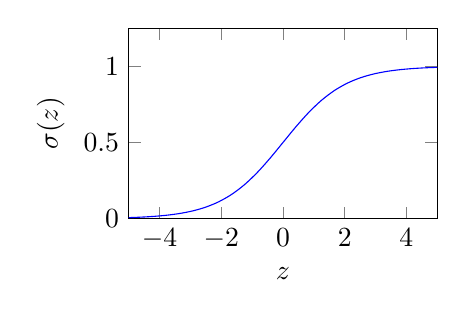
\begin{tikzpicture}
            \begin{axis}[width=5.5cm,height=4cm,ylabel=$\sigma(z)$,xlabel=$z$,ymin=0,ymax=1.25,xmin=-5,xmax=5]
                \addplot[blue,smooth] {1/(1+exp(-x))};
                %\addlegendentry{$y = \dfrac{1}{1+e^{-x}}$}
            \end{axis}
        \end{tikzpicture}
    }
        \caption[Funciones de activación]{}
        \label{fig:sigmoid-tanh}
\end{figure}


La función logistica estandar centrada en el origen como en la figura \ref{fig:graficaLog1} se escribe de la siguiente forma:
\begin{equation}
 \sigma(z) = \dfrac{1}{1+e^{-(z)}}
\end{equation}

Los siguientes calculos son realizados para un solo perceptrón, en concreto uno de salida, donde este está recibiendo los datos de salida de neuronas en la capa oculta, así el factor $z$ que está recibiendo la función, es la combinación lineal de los valores de entrada multiplicados por los pesos asignados para esté perceptrón y sumados todos. Entonces $z = X\Theta = [X_0\theta_0 +X_1\theta_1+...+X_n\theta_n]$. Así nuestra función queda de la siguiente forma:

\begin{equation}
  \sigma_{\Theta}(X) = \dfrac{1}{1+e^{-X\Theta}}
\end{equation}

Entonces vamos a calcular la derivada de esta función con respecto a cualquiera de estos parámetros $i$ de $z$.
Por la regla de la cadena comenzamos calculando la derivada queda de la siguiete forma:

\begin{equation}
 \dfrac{\partial\sigma}{\partial\theta_{i}}= -\dfrac{1}{(1-e^{-X\Theta})^2}e^{-x\Theta}(-x_{i})
\end{equation}

Reescribiendo la misma derivada con un poco de algebra nos queda de la siguiete forma:
\begin{equation}
 \dfrac{\partial\sigma}{\partial\theta_{i}}= \dfrac{1}{1+e^{-X\Theta}}  \dfrac{e^{-x\Theta}}{1+e^{x\Theta}} x_{i}
\end{equation}

Con la reescritura anterior nos damos cuenta que tenemos la función sigma en uno de los productos así que procedemos a sustituirlo y a sumar y restar unos unos. Así obteniendo lo siguiente:
\begin{equation}
 \dfrac{\partial\sigma}{\partial\theta_{i}}= \sigma_{\Theta}(X)\dfrac{e^{-x\Theta}-1+1}{1+e^{x\Theta}} x_{i}
\end{equation}

Vamos a separar a conveniencia los terminos de la siguiente forma:
\begin{equation}
 \dfrac{\partial\sigma}{\partial\theta_{i}}= \sigma_{\Theta}(X)
 \left( \dfrac{1+e^{-x\Theta}}{1+e^{-x\Theta}}-\dfrac{1}{1+e^{-x\Theta}}\right)x_{i}
\end{equation}

Así sustituyendo con la función sigmoide y llevando a uno, llegamos a lo siguiente:
\begin{equation}
 \dfrac{\partial\sigma}{\partial\theta_{i}}= \sigma_{\Theta}(X)
 (1- \sigma_{\Theta}(X))x_{i}
\end{equation}

Entonces lo que tenemos es una propiedad bastante interesante de la función logística. Se está calculando la derivada de sigma con respecto al exponente osea que sería:
Entonces lo que vemos es que la derivada de la sigmoide es la sigmoide por uno menos la sigmoide:

\begin{equation}
 \dfrac{\partial\sigma}{\partial\theta_{z}}= \sigma(1- \sigma)
\end{equation}


\begin{figure}[H]
 \centering
 \includegraphics[scale=0.5]{../Figuras/devLog.png}
 \caption{Gráfica de la derivada de la función logistica.}
 \label{fig:graficaLogDev}
\end{figure}

Las funciones logísticas se utilizan a menudo en redes neuronales para introducir no linealidad en el modelo o para sujetar señales dentro de un intervalo específico . Un elemento de red neuronal popular calcula una combinación lineal de sus señales de entrada y aplica una función logística limitada como función de activación al resultado; este modelo puede verse como una variante "suavizada" de la neurona umbral clásica .

Estas relaciones dan como resultado implementaciones simplificadas de redes neuronales artificiales con neuronas artificiales. Las funciones sigmoidales que son antisimétricas con respecto al origen (por ejemplo, la tangente hiperbólica) conducen a una convergencia más rápida cuando se entrenan redes con retropropagación.

Una opción común para la activación o "aplastamiento" funciones, usadas para grandes magnitudes para mantener la respuesta de la red neuronal limitada. 

Las funciones logísticas se utilizan en varios roles en estadística. Por ejemplo, son la función de distribución acumulativa de la familia logística de distribuciones y, un poco simplificadas, se utilizan para modelar la posibilidad que tiene un jugador de ajedrez de vencer a su oponente en el sistema de clasificación.

En la siguiente sección veremos la derivada de la función de error.

\section{Entrenamiento en la última capa}

En esta sección nos vamos a enfocar en la última capa de red, consideremos la siguiente red de la figura \ref{fig:REDuc}. 

\begin{figure}[H]
 \centering
 \includegraphics[scale=0.7]{../Figuras/AredNa.png}
 \caption{Red neuronal(entrenamiento última capa.)}
 \label{fig:REDuc}
\end{figure}

Vamos a calcular el gradiente considerando que estamos evaluando a la red para un ejemplar. Una vez que la red tomó los valores de entrada (neuronas en verde) y los evaluó pasando por la capa oculta (neuronas en azul) hasta asignar el ejemplar a una neurona de salida (neuronas en rojo). Lo que la función de error está midiendo es la \textit{distancia} entre lo que obtuvimos en la capa de salida y una colección de etiquetas objetivo, es decir, la clasificación real del ejemplar. 


Entonces por ahora nuestra función de error está actuando solo sobre la capa de salida, pero recordemos que para llegar a la evaluación de cualquiera de las neuronas en la capa de salida, se calculó la activación de la capa oculta y de la capa de entrada. Con los respectivos pesos de cada capa. Entonces podemos decir que los valores obtenidos en la evaluación final dependen directamente de los pesos en cada capa. 


Tomando en cuenta lo anterior, el gradiente lo vamos a calcular capa por capa. Desde la capa de salida hasta la capa de entrada.
Lo primero que tenemos que calcular es como dependió la función de error de los pesos de la capa oculta (azul) que la antecede.


La notación que vamos a usar más adelante va a considerar las neuronas de entrada con el índice $i$, las neuronas de la capa oculta con el índice $j$, y las neuronas de salida con el índice $k$. Así, los pesos que conectan a la neurona $j$ con la neurona $k$, se representan como $\theta_{jk}$. 


Para denotar la capa que estamos haciendo referencia vamos a emplear el superíndice $(L)$ con referencia a last, último en inglés, dado que estamos haciendo los cálculos desde la última capa, hacia atrás, la penúltima capa se va a indicar con $(L-1)$, la anterior de esta como $(L-2)$ y así sucesivamente. Entonces, para referirnos a un peso para la última capa, que conecta a la penúltima capa con la de salida, se escribe como $theta_{jk}^{L-1}$ que es el peso marcado en rojo en la figura \ref{fig:REDuc}.

Usemos la entropía cruzada como función de error, para un ejemplar \ref{entropiaCruzada}:
 \begin{equation}
  J (\Theta) = -\left[\sum_{k=1}^{s_{L}}y_{k}^{(i)} log(\textcolor{blue}{a_{k}^{(L)}}) + (1-y_{k}^{(i)}) log(1 - \textcolor{blue} {a_{k}^{(L)}})  \right] 
  \label{eq:EntropiaCruz}
 \end{equation}
 

 La suma está tomando en cuenta que el ejemplar puede ser clasificado a una de las varias clases a poder asignar $S_{L}$, es decir, el número de neuronas en la capa $L$. Los valores obtenidos de la activación las neuronas están definidos por $a_{k}^{(L)}$, y los deseados por $y_{k}$.
 
 Lo siguiente a hacer es calcular la derivada con respecto a los pesos que conectan la última capa con la penúltima capa, es decir, $\theta_{jk}^{(L-1)}$.
 
 Entonces vamos a calcular la parcial de error con respecto a uno de los pesos de la capa anterior. Así la suma se "va" dado que el peso solo va a afectar a la $k$-esima neurona, quedando solo con la operación que se efectúa en esta, usando la regla de cadena obtenemos lo siguiente:
 
 \begin{equation}
  \dfrac{\partial J}{\partial \theta_{jk}^{L-1}} = - \left[ \dfrac{y_{k}}{a_{k}^{L}} \dfrac{\partial}{\partial\theta_{jk}^{(L-1)}} g(\textcolor{red}{z_{k}}) - \left(\dfrac{1 - y_{k}}{1 - a_{k}^{L}} \right) \dfrac{\partial}{\partial \theta_{jk}^{(L-1)}}g(\textcolor{red}{z_{k}})\right]
 \end{equation}
 
Con:
\begin{equation}
 \textcolor{red}{z_{k}} = \sum_{j'=0}^{S_{L-1}} \theta_{j'k}a_{j'}^{L-1}
\end{equation}

Recodemos que $a_{k}^{(L)}$ está calculado por una función de activación $g(z_{k})$. Donde $z_{k}$ es la suma de las combinaciones lineales de las neuronas conectadas hacia la neurona $k_{n}$. Estos valores son calculados en el algoritmo de propagación hacia adelante. Los escribimos aquí para recodar como está siendo calculada la parcial.

De la derivada de la suma sólo queda $a_{j'} $ con $j' = j$. Siguiendo la regla de la cadena para los términos que nos faltaba nos queda lo siguiente:

\begin{equation}
 \dfrac{\partial J}{\partial \theta_{jk}^{L-1}} =-\left[ \dfrac{y_{k}}{a_{k}^{(L)}} \textcolor{blue}{g'(z_{k})} -\left( \dfrac{1-y_{k}}{1-a_{k}^{(L)}} \right) \textcolor{blue}{g'(z_{k})}\right]a_{j}^{(L)}
\end{equation}

Simplificando, nos queda lo siguiente:

\begin{equation}
 \dfrac{\partial J}{\partial \theta_{jk}^{L-1}} =-\left[ \dfrac{y_{k}(1-a_{k}^{(L)})-a_{k}^{(L)}(1-y_{k})} {a_{k}^{(L)}(1-a_{k}^{(L)})} \right]\textcolor{blue}{g'(z_{k})} a_{j}^{(L)}
\end{equation}

Recordando que la derivada de la sigmoide queda como $g' = g (1 - g)$ tenemos que:
\begin{equation}
 \textcolor{blue}{g'(z_{k})} = a_{k}^{(L)}(1-a_{k}^{(L)})
\end{equation}

Así nos queda como: 
\begin{equation}
 \dfrac{\partial J}{\partial \theta_{jk}^{L-1}} = -\left[ \dfrac{y_{k}- y_{k}a_{k}^{(L)} - a_{k}^{(L)} + a_{k}^{(L)}y_{k} } {a_{k}^{(L)}(1-a_{k}^{(L)})} \right] a_{k}^{(L)}(1-a_{k}^{L}) a_{j}^{(L)}
\end{equation}

Y haciendo un poco de álgebra nos queda como:
\begin{equation}
 \dfrac{\partial J}{\partial \theta_{jk}^{L-1}} =  -a_{j}^{(L-1)})(y_{k}-a_{k}^{(L)})
\end{equation}

Representando a $(y_{k}-a_{k}^{(L)})$ como $\delta_{k}$ nos queda:

\begin{equation}
 \dfrac{\partial J}{\partial \theta_{jk}^{L-1}} =-a_{j}^{(L-1)})\delta_{k}
\end{equation}

Esta última notación con delta se usa pues con esto estamos representando el error que se cometió en la última capa, pues es la diferencia entre lo desado y lo que se obtuvo realmente.

Con esto ya sabemos calcular todas las parciales del error con respecto a los pesos hacia la última capa. En la siguiente sección seguimos con el cálculo para las siguientes capas.

\section{Parcial con respecto a los pesos en la última capa}
Vacio >:|



\section{Vectorización}
La red hasta este momento solo había sido representada mediante nodos, ahora vamos a hacer el uso de una notación en particular la cúal consta de matrices y vectores. Para generalizar nuestras fórmulas en la derivación matemática. %, del grediente se hizo considerando que tuviéramos un solo ejemplar de entrenamiento pero realmente vamos a entrenar a nuestra red con varios ejemplares. 

Consideremos todos los datos involucrados durante el entrenamiento:
\begin{enumerate}
 \item Hay $S_{L}$ neuronas de salida, para las cuales se calculará el error.
 \item Se puede calcular el promedio del gradiente para m ejemplares simultáneamente.
 \item Si escribimos los datos en forma matricial, es posible paralelizar estos cálculos utilizando operaciones de matrices.
\end{enumerate}
Denotemos nuevamente nuestra función de error:
 \begin{equation}
  J (\Theta) = -\dfrac{1}{m}\left[\sum_{i=1}^{m}\sum_{k=1}^{s_{L}}y_{k}^{i} log( h_{\Theta}(x^i))_{k}+(1-y_{k}^{i})log(1- h_{\Theta}(x^i))_{k}  \right]  
 \end{equation}

Ahora con nuestros datos en forma matricial:
\begin{equation}
X = 
\begin{pmatrix}
x_{0}^{(1)} & \cdots & x_{n}^{(1)}\\
\vdots & \ddots & \vdots\\
x_{0}^{(m)} & \cdots & x_{n}^{(m)}\\
\end{pmatrix}
\end{equation}


\begin{equation}
Y = 
\begin{pmatrix}
y_{0}^{(1)} & \cdots & y_{S_{L}}^{(1)}\\
\vdots & \ddots & \vdots\\
y_{0}^{(m)} & \cdots & y_{S_{L}}^{(m)}\\
\end{pmatrix}
\end{equation}


\begin{equation}
\Theta^{(l)} = 
\begin{pmatrix}
\Theta_{01} & \cdots & \Theta_{0s_{l}}\\
\vdots & \ddots & \vdots\\
\Theta_{(s_{(l-1)}1)} & \cdots & \Theta_{(s_{(l-1)}Sl)}\\
\end{pmatrix}
\end{equation}

Podemos reescribir:
\begin{equation}
 \delta_{k}^{(L)}=(y_{k}-a_{k}^{(L)})
\end{equation}

\begin{align*}
\delta_{k}^{(L)}&=(y_{k}-a_{k}^{(L)})           &  \Delta^{(L)}&=Y-A^{(L)}
\end{align*}

\begin{align*}
 \dfrac{\partial J}{\partial\theta_{jk}^{L-1}}&=-\dfrac{1}{m}\sum_{i=1}^{m}a_{j}^{(L-1)(i)}\delta_{k}^{(L)(i)}             &  \nabla^{(L-1)}&=-\dfrac{1}{m}\left(A^{(L-1)}\right)^{T} \Delta^{L}
\end{align*}

\begin{align*}
\delta_{j}^{(L-1)}&=\left(\sum_{k=1}^{s_{L}} \delta_{k}^{(L)}\theta_{jk}\right)g'(z_{j})           &  \Delta^{(L-1)}&=\Delta^{(L)}\left(\Theta_{[1:,:]}^{(L-1)}\right)^{T} \circ g'(Z^{(L-1)})
\end{align*}

\begin{align*}
 \dfrac{\partial J}{\partial\theta_{jk}^{L-2}}&=-a_{i}^{(L-2)}\delta_{j}^{(L-i)}             &  \nabla^{(L-2)}&=-\dfrac{1}{m}\left(A^{(L-2)}\right)^{T} \Delta^{L-1}
\end{align*}

Vectorización 3

Las fórmulas vectorizadas se pueden escribir en forma general con: \emph{Error cometido por la última capa L.}
\begin{equation}
 \Delta^{(L)} = Y-A^{(L)}
\end{equation}

\emph{Error cometido por cualquier capa l − 1.}
\begin{equation}
  \Delta^{(L-1)}=\Delta^{(L)}\left(\Theta_{[1:,:]}^{(L-1)}\right)^{T} \circ g'(Z^{(L-1)})
\end{equation}

\begin{equation}
 g' (Z^{(l-1)}) = A^(l-1) \circ (1-A^{(l-1)})
\end{equation}

Componentes del gradiente con respecto a los pesos en $\Theta^{l-1}$.
\begin{equation}
  \nabla^{(L-1)}=-\dfrac{1}{m}\left(A^{(L-1)}\right)^{T} \Delta^{L}
\end{equation}

Nuestra formula de error, es un promedio de la suma de errores que se tuvo en cada ejemplar $(i)$ del total de ejemplares $m$.
Para poder empezar a trabajar con matrices vamos a empezar a ver cómo están escritos nuestros datos todo recordemos como habíamos dicho que íbamos a escribir nuestras entradas de entrenamiento la idea es que cada ejemplar es un renglón tenemos n características, está pensando en que estamos agregando aquí los sesgos y después  lo que ocurre con nuestras etiquetas de clasificación recordemos que en redes neuronales utilizamos el one hot en coding. Entonces aunque si tenemos cinco clases tenemos cinco neuronas de salida y eso quiere decir que nuestra etiqueta tiene algo así este sería una etiqueta en la que la clase correcta es la que está en la tercera neurona otro ejemplar podría ser de esta manera y pues aunque solamente haya uno que sea distinto de cero la forma en la que van a venir empaquetadas nuestras respuestas correctas va a ser precisamente en forma de matriz donde tenemos sobre los renglones tantos bits como neuronas haya en la última capa y tenemos hacia abajo los m ejemplares de entrenamiento después recordemos cómo teníamos escritas las matrices de pesos teníamos por cada columna los pesos que contribuyen a la a una neurona en la siguiente capa entonces sobre cada renglón tendríamos a tener tantos pesos como neuronas haya en la capa cl y hacia abajo vamos a tener tantos pesos como neuronas había en la capa $sl -1$ y que contribuyeron al siguiente elemento en ese l .
Así que tendríamos a las diferentes neuronas que van a estar en nuestra nueva capa eso es lo que va a hacer es que cuando multipliquemos x y z nos queden otra vez los valores de cada en la siguiente capa con los renglones correspondientes a los ejemplares de entrenamiento y horizontalmente los valores de activación de cada neurona en la siguiente bien entonces partes importantes ejemplares de entrenamiento hacia abajo para estos dos aquí el décima capa hacia acá está para l menos uno ahora están copiadas acá del lado izquierdo las fórmulas tal y como las obtuvimos ejemplar por ejemplar y lo que vamos a hacer ahora es escribirlas en forma matricial bueno que ya me adelanté ya se las escribí entonces va a ser más fácil. Lo que estamos viendo aquí para eso voy a utilizar ahora otro programa y aquí está vamos a utilizar aquí para que pueda dibujar qué es lo que está primero que teníamos en delta está en la capa no en la capa l bueno voy a dibujar aquí ahorita una pequeña red neuronal en este conector y entonces nos estamos preguntando por qué pasa con él aquí está él bueno lo que decíamos era que vamos a tener una de estas del estás por cada uno de nuestras neuronas de salida y lo que vamos a ver es qué tenemos los ejemplares hacia abajo y las neuronas horizontales los valores que tengo aquí verticalmente los acosté y es lo que tengo acá ya vimos también entonces que la llega realmente tiene varios bits horizontalmente y la sas también entonces si yo restó enrique menos acá observen que esto en realidad es un vector tengo una componente por cada neurona de salida entonces aunque aquí les saquemos componente por componente pues tengo uno de cada uno. 
El hacer las combinaciones de todos contra todos es cuando obtengo el efecto que ocurrió con cada peso pero quiero sumar estos productos para todos los ejemplares de entrenamiento y sumarlos bueno eso es prácticamente lo que hace una multiplicación de matrices ahora para poder hacer todo esto en un solo paso lo que tenemos que hacer es acomodar las acorde mente nos vamos a hacer lo siguiente ya habíamos dicho que esta delta que realmente tiene forma de matriz como ésta de tal manera que mira aquí hacia acá tenemos todos los es el es y así aquí abajo tenemos todos nuestros ejemplares de entrenamiento bueno y que sabemos de la aj y también son los valores de activación y queremos combinar cada j de cada ejemplar de entrenamiento con su respectiva que del mismo ejemplar de entrenamiento y después multiplicarlos y sumarlos bien entonces vamos a acomodar a la sas de la siguiente manera y vamos a poner hacia acá a los ejemplares de entrenamiento y así acá a los elementos son ordenadas iba a suceder si yo hago esto observen que se multiplican ejemplares de entrenamiento contra ejemplares de entrenamiento misma aj contra mismos del tak as pero de diferentes ejemplares de entrenamiento cada uno con su respectivo y además se suman para definir la coordenada que va a quedar aquí cuando yo tomé este contra la siguiente columna entonces otra vez vamos a estar multiplicando en ejemplares contra mi ejemplares los vamos a sumar y nos va a dar el dato que tengamos aquí los conservamos las columnas que teníamos acá s l cuando empiece a hacerlo con los renglones voy a tener entonces lo que ocurre con las s menos el c lm no son tan clones que teníamos acá y esto es sumamente interesante porque esto que está aquí debería de resultarnos un poco conocido sl sl - solo vamos a ver que teníamos acá sl sl - 1 tiene exactamente la misma forma en la matriz de pesos y no es coincidencia recordemos que es lo que estamos tratando de calcular estamos tratando de calcular el gradiente el ingrediente es la parcial con respecto a cada uno de los pesos entonces lo que acabamos de obtener es ese gradiente que tiene acomodadas cada una de las parciales en la posición que corresponde al mismo peso pero en la matriz de pesos bastante bonito muy bien entonces por eso cuando ponemos la matriz a él pero transpuesta para que tengamos ahora si los ejemplares de entrenamiento de forma horizontal. 

Entonces podemos obtener en una multiplicación de matriz todos los componentes del gradiente para los pesos en esa capa lo que ocurre con las siguientes bueno de hecho con los siguientes gradientes es que se van a hacer exactamente igual lo único que nos queda ligeramente entretenido es cómo vamos a calcular los errores de las capas intermedias hay entonces que observar lo siguiente en primer lugar las ventas van a tener la misma forma que éste es que primas entonces simple y sencillamente van a ser dos matrices donde se tienen que multiplicar componentes a componentes las vamos a poner con este símbolo que significa circo digo se llama cirque y significa multiplicación componente a componente entre estas dos matrices ahora como vamos a escribir ésta se parece a lo anterior pero ahora sobre lo que queremos es sumar es sobre las neuronas de salida recordemos que la contribución al error de una neurona de la capa intermedia pues es la suma sobre los errores a los que contribuyó en todas las neuronas en la capa siguiente entonces del ejercicio anterior ya debemos de ver como pista en que si queremos hacer una suma sobre estos elementos pues como que esto es lo que vamos a tener que tener en la parte horizontal de la primera matriz y vertical de la segunda entonces de aquí empiezan a salir precisamente los tips de cómo escribir estas 2 estás deltas pues ya tienen automáticamente de manera horizontal lo que está ocurriendo con cada una de las neuronas entonces se quedan exactamente iguales y lo que estaba ocurriendo con los pesos es que entonces vamos a crear los componentes de ese l sobre los renglones los necesitamos tomar la transpuesta para que cumpla con esa condición y en principio y básicamente ya quedaría que ese entonces está en notación extraña que tenemos en la parte de abajo recordemos que si estamos utilizando sesgos si estamos utilizando sesgos tenemos una neurona en esta capa que no está conectada en nadie con nadie en la parte de atrás entonces no existen pesos que hayan hecho que las neuronas de acá contribuyan al error de esta ésta no tenía error es un sesgo entonces aquí no hay nada que calcular por eso lo que tenemos que hacer en la parte de aquí es quitar a los elementos que corresponderían a las así pues el hecho de que los riesgos no están conectados con la capa anterior es básicamente lo que nos está diciendo es que quitemos de la matriz de pesos a todas las conexiones que parten de esta neurona porque estas conexiones pues no bueno ésta no va a estar contribuyendo cada día más bien las que estén en esta capa no están contribuyendo al error de esta neurona entonces lo que ocurra con esta neurona. 
Finalmente para los componentes del gradiente  lo único que vamos a hacer era multiplicar los valores de activación de la capa anterior por los errores de la capa siguiente y eso nos iba a dar ahora sí la participación del gradiente para cada uno de los pesos y esto lo podemos repetir obteniendo uno de una matriz de estos por cada matriz de pesos que hayamos utilizado los con esta técnica básicamente obtenemos el gradiente de pequeños bloques hitos de material de matrices una matriz por cada matriz de pesos si quieren escribir el gradiente entonces como se escribe usualmente en cálculo es como un solo vector pues lo que hay que hacer es aplanar todas esas pequeñas matrices y poner cada una de las componentes en una componente del vector y nos va a quedar un vector gigantesco que tiene tantas tantas componentes como la suma de componentes en todas estas matrices bien y con eso quedaría todo. 
Lo que  se acaba de calcular es el gradiente y cuando nosotros hallamos descenso por el gradiente, lo que necesitamos es la dirección inversa, por eso el signo negativo. Entonces finalmente podemos decir en lo qué consiste el algoritmo de propagación hacia atrás, lo único que estamos haciendo es obtener los ejemplares de entrenamiento las respuestas correctas necesitamos saber cuántas que pasan vamos a inicializar nuestras matrices de errores con ceros bueno podremos hacer lo mismo también con las del gradiente empezamos en la haciendo feedforward que es lo que nos indican estas primeras líneas asignando nuestros datos de entrenamiento a la primera capa la capa de chocolate a partir de ahí utilizamos feedforward para ir calculando todos los valores de activación de las siguientes capas hasta llegar a la última y a partir de ese momento podemos empezar a trabajar ahora sí con el entrenamiento de la red. Tomar en cuenta que era lo que queríamos para sustituir en los cálculos de los errores y los gradientes con las fórmulas que tenemos en la parte de atrás y nos importó precisamente las etiquetas y ya que tenemos. Entonces podemos actualizar, ahora si nuestros pesos en paralelo tienen que actualizarse todos al mismo tiempo no para actualizar primero unos y después otros porque eso ya no es el gradiente en paralelo, tenemos que actualizar tomando los pesos que ya teníamos menos alfa por el gradiente de la función de error, repitiendo esto el suficiente número de veces. La idea es que eventualmente estos pesos nos permitan encontrar un mínimo de la función de error.

Así el algoritmo queda de la siguiente forma:
\begin{figure}[H]
 \centering
 \includegraphics[scale=0.8]{../Figuras/Algoritmo1.png}
 \caption{Algoritmo de retropropagación.}
 \label{fig:algoritmo}
\end{figure}



\chapter{Optimización del entrenamiento} 
\section{Problemas en redes profundas}

Hasta este momento ya se ha visto como modelar desde una neurona hasta una red neuronal propiamente, se ha visto como hacer la configuración de tal manera que nos clasifique ejemplares, así como detectar el error en los pesos asignados y ajustarlo para mejores resultados. Ahora al momento de modelar redes neuronales profundas (en inglés deep neuronal networks, \emph{DNN}) tenemos que aceptar que el cálculo de estás asignaciones y ajustes requieren tiempo de cálculo, así llegando al \emph{primer problema, el tiempo de computación}. Y ademas nos podemos encontrar con \emph{el problema del sobreaprendizaje} este aparece cuando tenemos demasiadas hipótesis válidas pero no de suficientes datos para poder descartar todas menos la correcta. 

Cuando ajustamos los parámetros de una red neuronal a los datos del conjunto de entrenamiento, no podemos diferenciar las características realmente útiles de las irrelevantes o de las debidas al muestreo del conjunto de entrenamiento, por lo que siempre estamos
expuestos al riesgo de sobreajuste (overfitting en inglés).


 Métodos de regularización o la disminución de pesos  o la dispersión, se puede aplicar durante el entrenamiento para combatir el sobreajuste. Alternativamente, la regularización de dropout, omite aleatoriamente neuronas de las capas ocultas durante el entrenamiento. . Finalmente, los datos se pueden aumentar a través de métodos como el recorte y la rotación, de modo que los conjuntos de entrenamiento más pequeños se pueden aumentar de tamaño para reducir las posibilidades de sobreajuste.

Las DNN deben considerar muchos parámetros de entrenamiento, como el tamaño (número de capas y número de unidades por capa), la tasa de aprendizaje y los pesos iniciales. El barrido a través del espacio de parámetros para obtener parámetros óptimos puede no ser factible debido al costo en tiempo y recursos computacionales. Varios trucos, como el procesamiento por lotes (calcular el gradiente en varios ejemplos de entrenamiento a la vez en lugar de ejemplos individuales)  aceleran el cálculo, lo veremos más adelante. Las grandes capacidades de procesamiento de las arquitecturas de muchos núcleos (como GPU) han producido aceleraciones significativas en el entrenamiento.

Para mayor información del tema se sugiere leer el siguiente enlace:

CHAPTER 5 Why are deep neural networks hard to train? \url{http://neuralnetworksanddeeplearning.com/chap5.html}

El siguiente enlace les puede ayudar a ver como cada hiperparemetro puede afectar a los resultados de la red neuronal.
\url{https://quetzalcoatl.fciencias.unam.mx/moodle/mod/url/view.php?id=634&redirect=1}

Para ayudarnos a los calculos con el gradiente vea los siguientes enlaces:
\begin{itemize}
 \item \url{https://youtu.be/nUUqwaxLnWs}
 \item \url{https://youtu.be/FDCfw-YqWTE}
 \end{itemize}


\section{Gradiente desvaneciente (o que explota)}

Vacio.

\section{Entrenamiento en línea vs en lotes}

Las varias formas de entrenar son dependiendo de los objetivos, ahora en está sección veremos entrenamiento en linea y por lotes.

\begin{figure}[H]
 \centering
 \includegraphics[scale=0.8]{../Figuras/AredN.png}
 %\caption{última capa.}
 \label{fig:graficaLog}
\end{figure}

\section{Normalización y normalización por lotes}

Un factor importante a tomar en cuenta para un buen desempeño del entrenamiento son las magnitudes del datos de entrada a la red. Entonces para mejorar el desempeño del algoritmo de optimización nos conviene pre-procesar los datos de entrada. Esto mediante una técnica que se llama normalización (\emph{normalization} en inglés).

La técnica que hemos utilizado son técnicas de optimización basadas en el gradiente, la cual a una función de error se calcula el gradiente, este nos da la dirección del máximo descenso, para  hacer aproximaciones discretas en los parámetros hasta que tratemos de llegar al mínimo de la función.
 
Para poder realizar lo anterior necesitamo que las magnitudes de los datos de entrada no esten muy dispersas, es decir que no nos encontremos con situaciones donde estemos manejando decimales para unos datos y para otros unidades de millones. En estos casos la función de error nunca va a terminar de ajustarse correctamente a estos datos, pues en ocaciónes los parametros para ajustar, van a avanzar de forma distorsionada. Dando la impresión que para unos datos el gradiente avanza muy rapido al centro, mientras que para otros datos avanza muy lento, esto porque vamos a tener curvas de nivel demasiado elípticas (ver la figura \ref{fig:curvasNivel}), entonces al tomar la dirección que nos de el gradiente, nos va a mover desplazar muy violentamente en algunas y muy lento para otras. Cuando se intente hacer descenso por el gradiente en estas regiones lo que va a pasar es que el vector va a oscilar muy violentamente y  nos va a dificultar mucho llegar al minimo.

Por el contrario, si las magnitudes con las que trabajamos son del mismo orden y contribuyen numéricamente de una manera más proporcionada al error, entonces vamos a tener curvas de nivel  más circulares (ver la figura \ref{fig:curvasNivel}). Cuando calculemos el gradiente, la perpendicular se aproximará durante más tiempo a la dirección de máximo descenso. 

\begin{figure}[H]
 \centering
 \includegraphics[scale=0.5]{../Figuras/curvasDeNivel.png}
 \caption{Izq: J la función de error con alta excentricidad. Der: J con curvas de nivel tendiendo a círculos}
 \label{fig:curvasNivel}
\end{figure}

Entonces para asegurar un buen desenso por el grandiente, vamos a preferir siempre trabajar con curvas de nivel circulares, para esto vamos a usar la normalización.

La normalización conciste en centrar los datos aproximadamente en el intervalo $[-1.0, 1.0]$, este intervalo no es estricto para todas las redes basta con definir las magnitudes en un intervalo aceptable para tener curvas de nivel circulares. 

Existen varias fórmulas para realizar la normalización, se sugiere la siguiente forma:
\begin{itemize}
 \item Calcular \emph{la media} $\mu_i$ y \emph{varianza} $\sigma_{i}^2$ para cada característica $i$ en los datos del conjunto de entrenamiento $X$.
 \begin{itemize}
  \item Las formulas son las siguientes, con $X_i$ la columna con la i-ésima característica en los datos de entrenamiento $X$.\\
  \begin{equation}
   \mu_{i} = \dfrac{1}{m}\sum_{i=1}^{m}x_{i} 
  \end{equation}
  \begin{equation}
   \sigma_{i}^{2} = \dfrac{1}{m}\sum_{i=1}^{m}(x_{i}-\mu)^2 
  \end{equation}
  \begin{equation}
   X_{i} = \dfrac{X_{i}-\mu}{\sigma^{2}}
  \label{eq:tres}
  \end{equation}
 \end{itemize}
    \item La media es el promedio de los datos de entrada.
    \item La varianza es una medida de dispersión, para ver que tan separados estan los datos unos de otros.
    \item La reasignación para cada $X_i$ va a ser, la resta $X_i -\mu$, que va a centrar los datos alrededor del cero, y la división por la varianza $\sigma^2$ que va a encoger los intervalos de distancia entre los datos. 
\end{itemize}

 
\begin{itemize}
 \item Una vez que la red se entreno con datos normalizados, \textit{es necesario almacenar las medias y varianzas} utilizadas durante el entrenamiento con el conjunto de entrenamiento $X$.
 \item Estos valores serán utilizados para normalizar datos nuevos que vayan a ser evaluados en la red. Esto para evitar que los nuevos datos usen magnitudes fuera del intervalo usado durante el entrenamiento de la red.
\end{itemize}

\begin{definition}
 \emph{La normalización} permite reducir la excentricidad en la función de error provocada por la disparidad entre los datos de entrada.
\end{definition}
  
 Entonces ya tenemos resuelta la situación de la disparides entre los datos de entrada. Ahora tenemos que, al calcular los valores para las capas intermedias, los valores pueden cambiar sus rangos para las neuronas intermedias. Para esta situación tenemos la normalización por lotes (\emph{bach normalization} en inglés).
 
La normalización por lotes aplica los beneficios de la normalización a las capas intermedias, haciendo que estás den valores en intervalos no muy grandes para las siguientes capas.

Una ventaja que nos da esta herramienta es que los algoritmos de optimización podrán utilizar \textit{tazas de aprendizaje más altas}, porque los brincos discretos del algoritmo no cambiarán drásticamente el comportamiento de la función de error durante un intervalo más largo.

Otra ventaja es que al normalizar entre capas, permite que cada capa calcule características distintas, independientemente que se otorguen ejemplares con mucho sesgo en una característica en especial. Permitiendo una mejor clasificación aún con datos nuevos. 

\begin{definition}
 La \emph{normalización por lotes} conciste en: 
 \begin{enumerate}
  \item  Normalizar la salida de la capa de activación anterior restando su media y dividiendo entre la desviación estándar.
  \item Hacer descenso por el gradiente estocástico.
  \item Dos paremetros: $\gamma$ una desviación estandar y $beta$ una media para corrimiento.
 \end{enumerate}
\end{definition}

Cuando se use el descenso por el gradiente estocástico (el descenso por el gradiente por lotes) modificará los pesos para optimizar $J$ la función de error, y probablemente contrarreste el efecto de la normalización.
Para evitarlo, se añaden dos parámetros, también entrenables: $\gamma$ una desviación estándar y $\beta$ una media para corrimiento, la idea es que el algoritmo tienda a
modificar estos dos para ese fin, en lugar de los pesos, de modo que los pesos produzcan un cómputo más estable.

Entonces la idea concreta es que dado un $B$ el minilote con $x_i$ sus ejemplares, las entradas $y_i$ para la capa siguiente se
calculan con las formulas:
  \begin{equation}
   \mu_{B} = \dfrac{1}{m}\sum_{i=1}^{m}x_{i} 
  \end{equation}
  \begin{equation}
   \sigma_{B}^{2} = \dfrac{1}{m}\sum_{i=1}^{m}(x_{i}-\mu_{B})^2 
  \end{equation}
  \begin{equation}
   x_{i} = \dfrac{X_{i}-\mu_{B}}{ \surd \sigma_{B}^{2} + \varepsilon}
  \label{eq:tres}
  \end{equation}
  \begin{equation}
   y_{i} = \gamma x_{i}+\beta \equiv BN_{\gamma,\beta}(x_{i})
  \label{eq:tres}
  \end{equation}

con $\varepsilon$ una constante agregada para mantener la estabilidad numérica.

\input{secciones/cap7/05Regularización}

\chapter{Caso de análisis e interpretación}
\section{Red Hinton árbol familiar con numpy (entrenamiento)}

En esta sección vamos a ver un ejemplo propuesto por Geoffrey Hinton, en el artículo \emph{Aprendiendo representaciones distribuidas de conceptos}, donde el objetivo es que una red neuronal aprenda el parentesco entre familiares, y para la creación de esta, se ayuda de lo que conocemos como árboles familiares.

\section{Red Hinton árbol familiar con pytorch}
Vacio.


\chapter{Entrenamiento con genéticos}
%\section{MNIST versión básica con numpy}
\section{Algoritmos genéticos}

Un algoritmo genético, conciste en  ``evolucionar'' una población de individuos, cada uno de los cuales representa una posible solución. Esa población se somete a la evolución biológica es decir mutaciones y recombinaciones genéticas. De generación en generación, los individuos se seleccionan de acuerdo con una función de adaptación o \emph{fitness}, en función de la cual se decide qué individuos sobreviven los más aptos y son descartados los menos aptos.

La selección se realiza siempre de forma probabilística. Un individuo es más probable que se seleccione si tiene un mejor valor de fitness, aunque cualquier individuo, por malo que sea, tiene una probabilidad de selección estrictamente mayor que cero. En ocasiones, si no queremos que una muy buena solución encontrada en una generación intermedia
de la evolución se pierda por el camino, podemos introducir cierto grado de elitismo en la selección. Podemos hacer que el mejor individuo de la población (o los k mejores) siempre sobrevivan, algo que aleja a los algoritmos genéticos del mundo real, donde una generación termina siempre reemplazando por completo a las anteriores.

\input{secciones/cap9/02Neuroevolución}
\subsection{Antecedentes: Aprendizaje por refuerzo en videojuegos}
Vacio.

\subsection{Arquitectura para estimar la función de recompensa}
Vacio.

\input{secciones/cap9/023Entrenamiento}

%\part{Aprendizaje no supervisado}
\chapter{Mapeos autoorganizados}
\input{secciones/cap10/00Introducción}
\section{Aprendizaje no supervisado}
Vacio.

\section{Mapeos autoo-organizados}
Vacio.

\input{secciones/cap10/03Kohonen}

%%
%\part{NO TIENE NOMBRE}
\chapter{Redes Neuronales Convolucionales}
\section{Convolución}
\section{Redes Convolucionales}
\section{Softmax}
\section{MNIST}

%%
\part{Redes con ciclos}
\chapter{Redes Neuronales Recurrentes}
\section{Derivadas ordenadas}
\section{Retropropagación en el tiempo}
\section{Sistemas dinámicos y despliegue del grafo}
\section{Arquitectura recurrente universal}
\section{Función de error}
\section{Forzamiento del profesor}

\chapter{Atención}
%\section{Casos de análisis de serie}
\chapter{LSTM}
\chapter{GRU}
\chapter{Casos de análisis: etiquetado de palabras y conjugación de verbos}

\part{Redes no dirigidas}
\chapter{Redes de hopfield}
\section{Entrenamiento}

\chapter{Máquinas de Boltzman}
\section{Entrenamiento}
\subsection{Partículas y partículas de fantasía}
\subsection{Máquinas de Boltzman Restringidas}

\chapter{Redes adversarias}
\section{GANs}

\appendix 
\chapter{Ecuaciones diferenciales}

%----------------------------------------------------------------------------------------
% Bibliografia
%----------------------------------------------------------------------------------------
\backmatter

\printbibliography[heading=bibintoc]

\end{document}
